%%%%%% Run at command line, run
%%%%%% xelatex grad-sample.tex 
%%%%%% for a few times to generate the output pdf file
\documentclass[12pt,oneside,openright,a4paper]{cpe-english-project}

\usepackage{polyglossia}
\usepackage{float}
\setdefaultlanguage{english}
\setotherlanguage{thai}
\newfontfamily\thaifont[Script=Thai,Scale=1.23]{TH Sarabun New}
\defaultfontfeatures{Mapping=tex-text,Scale=1.0,LetterSpace=0.0}
\setmainfont[Scale=1.0,LetterSpace=0,WordSpace=1.0,FakeStretch=1.0]{Times New Roman}
\emergencystretch=10pt
%\XeTeXlinebreaklocale "th_TH"	
%\XeTeXlinebreakskip = 0pt plus 1pt
%\setmathfont(Digits)[Scale=1.0,LetterSpace=0,FakeStretch=1.0]{Times New Roman}

%%%%%%%%%%%%%%%%%%%%%%%%%%%%%%%%%%%%%%%%%%%%%%%%%%%%%%%%%%%%%%%%%%%
% Customize below to suit your needs 
% The ones that are optional can be left blank. 
%%%%%%%%%%%%%%%%%%%%%%%%%%%%%%%%%%%%%%%%%%%%%%%%%%%%%%%%%%%%%%%%%%%
% First line of title
\def\disstitleone{Generative AI for Traditional Form Converter}   
% Second line of title
% \def\disstitletwo{Project/Indep title line 2 (optional)}   
% Your first name and lastname
\def\dissauthor{Mr. PRAPAKORN BUTYOJANTO}   % 1st member
\def\dissauthortwo{Mr. PHANASORN SRISAYAM}   % 2nd member (optional)
\def\dissauthorthree{Mr. NATTAWUT PIANOK}   % 3rd member (optional)


% The degree that you're persuing..
\def\dissdegree{Bachelor of Engineering} % Name of the degree
\def\dissdegreeabrev{B.Eng} % Abbreviation of the degree
\def\dissyear{2024}                   % Year of submission
\def\thaidissyear{2567}               % Year of submission (B.E.)

%%%%%%%%%%%%%%%%%%%%%%%%%%%%%%%%%%%%%%%%%%%%
% Your project and independent study committee..
%%%%%%%%%%%%%%%%%%%%%%%%%%%%%%%%%%%%%%%%%%%%
\def\dissadvisor{Dr. Kittipong Piyawanno , Ph.D.}  % Advisor
%% Leave this empty if you have no co-advisor
\def\disscoadvisor{} %Optional
\def\disscommitteetwo{Assoc.Prof. Natasha Dejdumrong, D.Tech.Sci.} 
\def\disscommitteethree{Assoc.Prof. Peerapon Siripongwutikorn, Ph.D.}  
\def\disscommitteefour{Naveed Sultan} 

\def\worktype{Project} %%  Project or Independent study
\def\disscredit{3}   %% 3 credits or 6 credits


\def\fieldofstudy{Computer Engineering} 
\def\department{Computer Engineering} 
\def\faculty{Engineering}

\def\thaifieldofstudy{วิศวกรรมคอมพิวเตอร์} 
\def\thaidepartment{วิศวกรรมคอมพิวเตอร์} 
\def\thaifaculty{วิศวกรรมศาสตร์}
 
\def\appendixnames{Appendix} %%% Appendices or Appendix

\def\thaiworktype{ปริญญานิพนธ์} %  Project or research project % 
\def\thaidisstitleone{เว็บแอปพลิเคชัน AI สำหรับการแปลงฟอร์มกระดาษเป็นเว็บฟอร์ม}
\def\thaidissauthor{นายประภากร บุตรโยจันโท}
\def\thaidissauthortwo{นายพณศร ศรีสยาม} %Optional
\def\thaidissauthorthree{นายณัฐวุฒิ เพียนอก} %Optional

\def\thaidissadvisor{ดร. กิตติพงษ์ ปิยะวรรณโณ}
%% Leave this empty if you have no co-advisor
\def\thaidisscoadvisor{} %Optional
\def\thaidisscoadvisortwo{}  % Co-advisor 2 (if any)
\def\thaidisscoadvisorthree{} % Co-advisor 3 (You better be building space rocket or curing cancer at this point)
\def\thaidissdegree{วิศวกรรมศาสตรบัณฑิต}

% Change the line spacing here...
\linespread{1.15}

%%%%%%%%%%%%%%%%%%%%%%%%%%%%%%%%%%%%%%%%%%%%%%%%%%%%%%%%%%%%%%%%
% End of personal customization.  Do not modify from this part 
% to \begin{document} unless you know what you are doing...
%%%%%%%%%%%%%%%%%%%%%%%%%%%%%%%%%%%%%%%%%%%%%%%%%%%%%%%%%%%%%%%%


%%%%%%%%%%%% Dissertation style %%%%%%%%%%%
%\linespread{1.6} % Double-spaced  
%%\oddsidemargin    0.5in
%%\evensidemargin   0.5in
%%%%%%%%%%%%%%%%%%%%%%%%%%%%%%%%%%%%%%%%%%%
%\renewcommand{\subfigtopskip}{10pt}
%\renewcommand{\subfigbottomskip}{-5pt} 
%\renewcommand{\subfigcapskip}{-6pt} %vertical space between caption
%                                    %and figure.
%\renewcommand{\subfigcapmargin}{0pt}

\renewcommand{\topfraction}{0.85}
\renewcommand{\textfraction}{0.1}

\newtheorem{theorem}{Theorem}
\newtheorem{lemma}{Lemma}
\newtheorem{corollary}{Corollary}

\def\QED{\mbox{\rule[0pt]{1.5ex}{1.5ex}}}
\def\proof{\noindent\hspace{2em}{\itshape Proof: }}
\def\endproof{\hspace*{\fill}~\QED\par\endtrivlist\unskip}
%\newenvironment{proof}{{\sc Proof:}}{~\hfill \blacksquare}
%% The hyperref package redefines the \appendix. This one 
%% is from the dissertation.cls
%\def\appendix#1{\iffirstappendix \appendixcover \firstappendixfalse \fi \chapter{#1}}
%\renewcommand{\arraystretch}{0.8}
%%%%%%%%%%%%%%%%%%%%%%%%%%%%%%%%%%%%%%%%%%%%%%%%%%%%%%%%%%%%%%%%
%%%%%%%%%%%%%%%%%%%%%%%%%%%%%%%%%%%%%%%%%%%%%%%%%%%%%%%%%%%%%%%%


\begin{document}
\pdfstringdefDisableCommands{%
\let\MakeUppercase\relax
}
\begin{center}
  
\includegraphics[width=2.8cm]{logo02.jpg}
\end{center}
\vspace*{-1cm}

\maketitlepage
\makesignaturepage 

%%%%%%%%%%%%%%%%%%%%%%%%%%%%%%%%%%%%%%%%%%%%%%%%%%%%%%%%%%%%%%
%%%%%%%%%%%%%%%%%%%%%% English abstract %%%%%%%%%%%%%%%%%%%%%%%
%%%%%%%%%%%%%%%%%%%%%%%%%%%%%%%%%%%%%%%%%%%%%%%%%%%%%%%%%%%%%%
\abstract

\setlength{\parindent}{15pt} Generative AI for Traditional Form Converter is a project developed through a web application called PaperlessTransform Application
to solve the problem of taking a long time to convert paper forms into web applications. The development of this web application uses artificial intelligence to analyze the types of data of questions.\par
As the demand for form conversion increases, system developers need to analyze forms and design database systems, design web application pages, and develop new systems.
This results in increased work time. In addition, system developers face increased workloads, causing personnel to spend inefficient time on their work.
Our project focuses on developing a web application that can convert documents in the form of paper forms or electronic files into web application formats.
It uses optical character recognition techniques to convert text images into text formats to process the text from the converted text images to detect questions in the form format.\par
The project team focuses on developing a web application that has the ability to detect questions and store web form data.
The aim is to reduce the burden on system developers. The results after testing the web application in the work show that the web application can detect questions in the form and store data at a satisfactory level. Therefore, it can be concluded that the project can significantly solve the problem of increased work time for system developers.

\begin{flushleft}
\begin{tabular*}{\textwidth}{@{}lp{0.8\textwidth}}
\textbf{Keywords}: & Web Application / Optical Character Recognition (OCR) / Database Design

\end{tabular*}
\end{flushleft}
\endabstract

%%%%%%%%%%%%%%%%%%%%%%%%%%%%%%%%%%%%%%%%%%%%%%%%%%%%%%%%%%%%%%
%%%%%%%%%% Thai abstract here %%%%%%%%%%%%%%%%%%%%%%%%%%%%%%%%%
%%%%%%%%%%%%%%%%%%%%%%%%%%%%%%%%%%%%%%%%%%%%%%%%%%%%%%%%%%%%%%
{
%\begin{thai}
\XeTeXlinebreaklocale "th_TH"	
\XeTeXlinebreakskip = 0pt plus 1pt
\thaifont
\thaiabstract

Generative AI for Traditional Form Converter เป็นโครงการที่จัดทำขึ้นผ่านการพัฒนาผ่านเว็บแอปพลิเคชั่นในชื่อ PaperlessTransform Application
เพื่อแก้ไขปัญหาการใช้ระยะเวลานานในการแปลงแบบฟอร์มกระดาษเป็นรูปแบบเว็บแอปพลิเคชัน โดยการพัฒนาเว็บแอปพลิเคชันนี้ได้มีการใช้ประยุกต์ใช้ปัญญาประดิษฐ์สำหรับการวิเคราะห์เกี่ยวกับประเภทของข้อมูลของคำถาม 
ตามความต้องการที่เพิ่มขึ้นของการแปลงแบบฟอร์ม ดังนั้นนักพัฒนาระบบจึงจำเป็นต้องวิเคราะห์แบบฟอร์มและออกแบบระบบฐานข้อมูลพร้อมทั้งการออกแบบหน้าเว็บแอปพลิเคชัน รวมไปถึงการพัฒนาระบบขึ้นมาใหม่
จึงส่งผลให้ต้องใช้ระยะเวลาในการทำงานที่เพิ่มขึ้น นอกจากนี้ นักพัฒนาระบบต้องเผชิญกับปัญหาภาระงานที่มากขึ้น ส่งผลให้บุคคลากรใช้เวลาในการทำงานอย่างไม่มีประสิทธิภาพ 
โดยโครงการของเรามุ่งเน้นการพัฒนาเว็บแอปพลิเคชันที่สามารถแปลงเอกสารในรูปแบบของฟอร์มกระดาษ หรือ ไฟล์อิเล็กทรอนิกส์ให้เป็นรูปแบบของเว็บแอปพลิเคชัน 
โดยใช้เทคนิคการรู้จดจำอักขระด้วยแสงในการแปลงภาพข้อความให้เป็นรูปแบบข้อความเพื่อนำข้อความดังกล่าวจากการแปลงภาพข้อความนำมาประมวลผลในการตรวจจับคำถามในรูปแบบฟอร์ม 
ทางคณะผู้จัดทำโครงการมีการเน้นการพัฒนาเว็บแอปพลิเคชันที่มีความสามารถในการตรวจจับคำถามและความสามารถในการเก็บข้อมูลของเว็บฟอร์ม 
โดยมีวัตถุประสงค์เพื่อลดภาระของนักพัฒนาระบบ โดยผลลัพธ์หลังจากมีการทดลองใช้เว็บแอปพลิเคชั่นดังกล่าวในการทำงานแสดงให้เห็นว่าเว็บแอปพลิเคชันสามารถตรวจจับคำถามในแบบฟอร์มและเก็บข้อมูลได้ในระดับที่น่าพึ่งพอใจ ดังนั้นสรุปได้ว่าโครงการสามารถแก้ไขปัญหาการใช้ระยะเวลาในการทำงานที่เพิ่มขึ้น ของนักพัฒนาระบบได้อย่างมีนัยสำคัญ

\begin{flushleft}
\begin{tabular*}{\textwidth}{@{}lp{0.8\textwidth}}
 & \\

\textbf{คำสำคัญ}: & เว็บแอปพลิเคชัน / การรู้จดจำอักขระด้วยแสง /  ออกแบบระบบฐานข้อมูล
\end{tabular*}
\end{flushleft}
\endabstract
%\end{thai}
}

%%%%%%%%%%%%%%%%%%%%%%%%%%%%%%%%%%%%%%%%%%%%%%%%%%%%%%%%%%%%
%%%%%%%%%%%%%%%%%%%%%%% Acknowledgments %%%%%%%%%%%%%%%%%%%%
%%%%%%%%%%%%%%%%%%%%%%%%%%%%%%%%%%%%%%%%%%%%%%%%%%%%%%%%%%%%
\preface
The authors would like to express special sincere gratitude to Dr. Kittipong Piyawanno, the project advisor,
who always supported and guided the project's direction throughout this project journey. His expertise and mentorship have played an important role in our project to shape the project. \par
Additionally, I would like to thank all the contributors across various platforms, such as Medium, Stack Overflow, and ChatGPT, whose shared knowledge and expertise have been invaluable. Their contributions have significantly enhanced my understanding and helped us refine our work. \par
Finally, we would like to express our thanks to everyone, including our family, friends, and everyone who has contributed and supported this project. All the support and encouragement have been integral to its successful completion.

%%%%%%%%%%%%%%%%%%%%%%%%%%%%%%%%%%%%%%%%%%%%%%%%%%%%%%%%%%%%%
%%%%%%%%%%%%%%%% ToC, List of figures/tables %%%%%%%%%%%%%%%%
%%%%%%%%%%%%%%%%%%%%%%%%%%%%%%%%%%%%%%%%%%%%%%%%%%%%%%%%%%%%%
% The three commands below automatically generate the table 
% of content, list of tables and list of figures
\tableofcontents                    
\listoftables
\listoffigures                      

%%%%%%%%%%%%%%%%%%%%%%%%%%%%%%%%%%%%%%%%%%%%%%%%%%%%%%%%%%%%%%
%%%%%%%%%%%%%%%%%%%%% List of symbols page %%%%%%%%%%%%%%%%%%%
%%%%%%%%%%%%%%%%%%%%%%%%%%%%%%%%%%%%%%%%%%%%%%%%%%%%%%%%%%%%%%
% You have to add this manually..
\listofsymbols
\begin{flushleft}
\begin{tabular}{@{}p{0.07\textwidth}p{0.7\textwidth}p{0.1\textwidth}}
\textbf{SYMBOL}  & & \textbf{UNIT} \\[0.2cm]
$\alpha$ & Test variable\hfill & m$^2$ \\
$\lambda$ & Interarival rate\hfill &  jobs/second\\
$\mu$ & Service rate\hfill & jobs/second\\
\end{tabular}
\end{flushleft}
%%%%%%%%%%%%%%%%%%%%%%%%%%%%%%%%%%%%%%%%%%%%%%%%%%%%%%%%%%%%%%
%%%%%%%%%%%%%%%%%%%%% List of vocabs & terms %%%%%%%%%%%%%%%%%
%%%%%%%%%%%%%%%%%%%%%%%%%%%%%%%%%%%%%%%%%%%%%%%%%%%%%%%%%%%%%%
% You also have to add this manually..
\listofvocab
\begin{flushleft}
\begin{tabular}{@{}p{1in}@{=\extracolsep{0.5in}}p{0.73\textwidth}}
AI & Artificial Intelligence\\
ML & Machine Learning  \\
NLP & Natural Language Processing  \\
OCR & Optical Character Recognition  \\
UX/UI & User Interface and User Experience
\end{tabular}
\end{flushleft}

%\setlength{\parskip}{1.2mm}

%%%%%%%%%%%%%%%%%%%%%%%%%%%%%%%%%%%%%%%%%%%%%%%%%%%%%%%%%%%%%%%
%%%%%%%%%%%%%%%%%%%%%%%% Main body %%%%%%%%%%%%%%%%%%%%%%%%%%%%
%%%%%%%%%%%%%%%%%%%%%%%%%%%%%%%%%%%%%%%%%%%%%%%%%%%%%%%%%%%%%%%


\chapter{Introduction}

\section{Problem Statement} 

In recent year, the world has become more digitized than ever, whether it be using electronic devices for note-taking instead of paper or storing a data in a database rather than use a paper documentation, However, there are still many aspects that have not been transform to be a digital, such as a government organization that still rely on paper documentation or  the data forms that have been previously recorded on paper. However, for those that have not been developed to be digital, we were motivated to improve the efficiency of form filling. And we found that the development process from paper-based forms to web forms required developers to do an analysis of the form, create a database, and develop a front-end and backend system. Which causes a developer time to spend and resources of developers. We acknowledge this difficulty and offer a solution that converts paper forms into web form ones so that the system can automatically create a web form by just taking a picture of the form. By decreasing excessive paper use, this development in digitizing form-filling procedures will not only increase efficiency but also lessen the environmental impact and help to slow down global warming.

\section{Objectives}
\begin{itemize}
\item   To reduce the workload and development process for developers. 
\item   To acquire the knowledge and skills necessary for developing an AI-powered web
application
\item To acquire proficiency in utilizing a Large language models and adapt its capabilities to suit the
requirements of this project.
\item  To be the secure all data and form management website
\end{itemize}

\section{Scope of Work}

The scope of this project involves the development of a web application that enables users to upload a PDF or image file. The web application will process text extraction using optical character recognition (OCR). The primary function of the web application includes creating a form, editing a form, deleting a form, and filling a form. The final deliverable of this project will be a responsive web interface web application that allows users to manage the form and view the data, including ensuring data privacy and security measures to protect sensitive information by implementing authentication for the creator and a normal user. The project involves research of optical character recognition (OCR) for the text extraction from the image and the development of generative AI for data type generation, also a Thai language translation to English.
%\begin{itemize}
%\item   What are the problems you are addressing? 
%\item  Why they are important?
%\item  What are the limitations of existing approaches? 
%\end{itemize}

\section{Limitation of Project}
The limitation of the project will addresses a possible constraints and challenges that might affect its scope, execution, or outcomes. the limiting factor are include time, cost and risk etc.

\begin{itemize}
 \item \textbf{OCR Accuracy:} The accuracy of OCR text extraction may vary depending on the quality of the uploaded document, such as low-resolution images, poor lighting, and the project does not support handwritten text.
 
    \item \textbf{Language Support:} While the system has the ability to translate text, the accuracy and availability of supported languages may be limited, with the project currently supporting Thai and English form only.
    
    \item \textbf{Required User Reviewing:} After the text extraction and layout detection, the system required a user to review and correct a input label that the system have process. The limitation required of user reviewing because of the lack of OCR accuracy and the system error.
      
    \item \textbf{Data Privacy and Security:} Despite the implementation of verification and security measures, there may still be vulnerabilities related to handling sensitive data, which are continuously checked and updated.
\end{itemize}


\section{Project Schedule}
For the first semester, our project focus on researching and design phase, We have researching all core fundamental concept and define a problem and background of the project. In the design phase, we have design a database design, UX/UI design, architecture design. And this phase also including a Optical Character Recognition proof of concept.

\begin{figure}[H]
\centering
\fbox{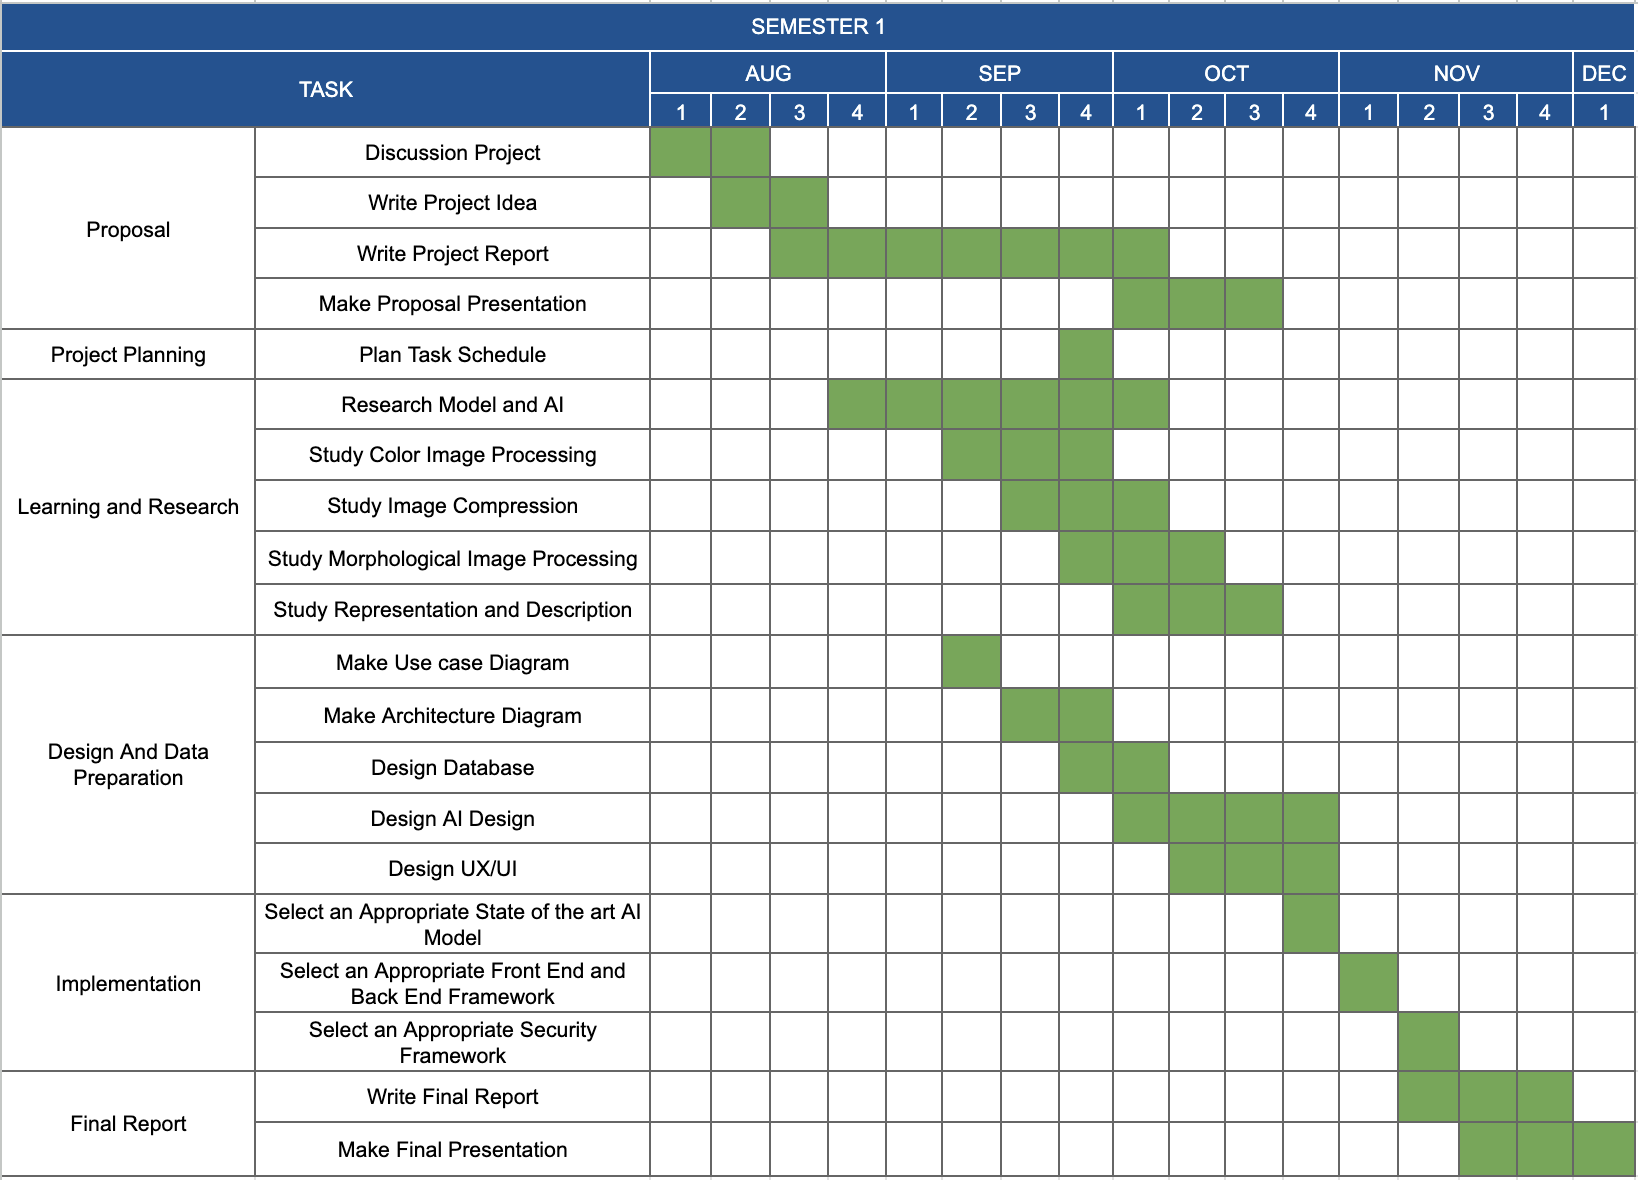
\includegraphics[width=10cm]{./assets/schedule-term1.png}}
\caption{Schedule for first semester}\label{fig:figure-1.1}
\end{figure}

For the second semester, our project focus on implementing the form extractor and generative AI for the process of detect a form. We also focus on web application development and integrate a web application with the form extractor. also including the testing phase a system evaluation.

\begin{figure}[H]
\centering
\fbox{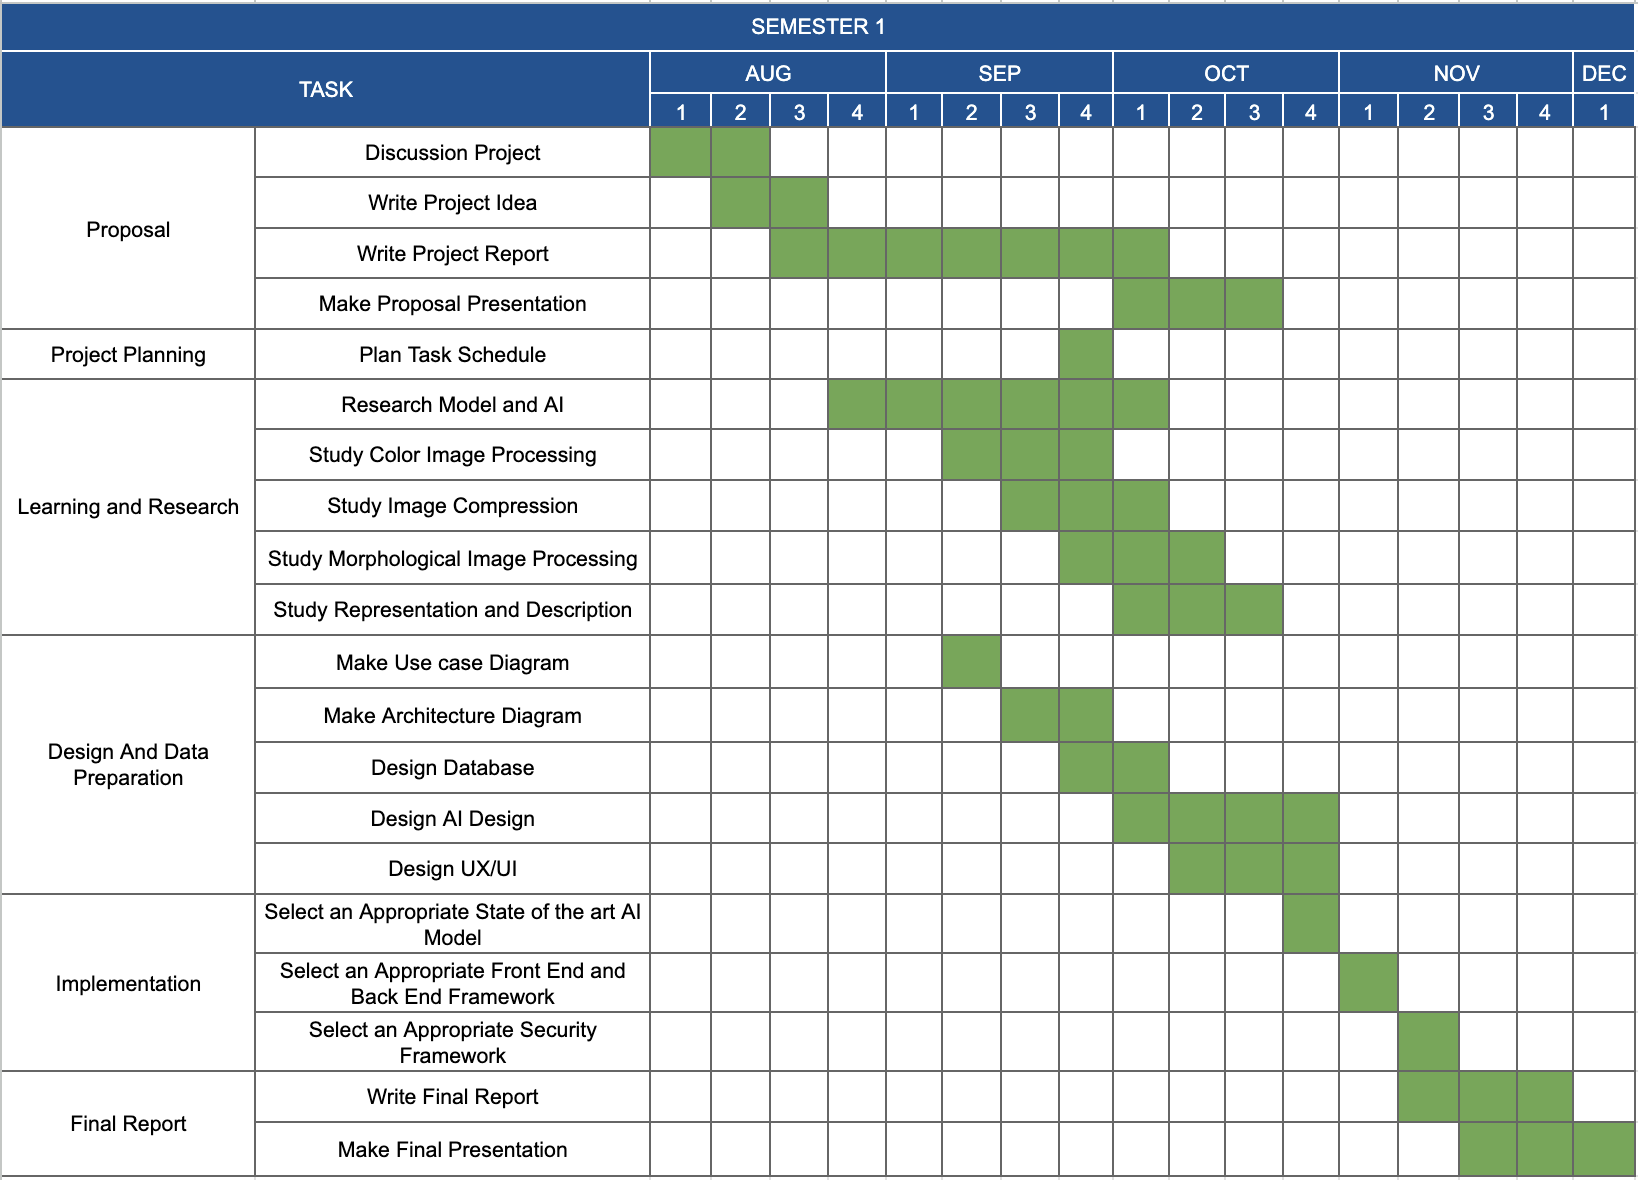
\includegraphics[width=10cm]{./assets/schedule-term1.png}}
\caption{Schedule for second semester}\label{fig:figure-1.2}
\end{figure}

\section{Expected Outcomes}
This project aims to develop a fully functional web application that able to converting a paper-based form or pdf form into a web-based form by utilizing a generative AI for generate a data type of form label. And the web application should reduce a time developer have spend when they converting a form.

%%%%%%%%%%%%%%%%%%%%%%%%%%%%%%%%%%%%%%%%%%%%%%%%%%%%%%%%%%%%
%%%%%%%%%%%%%%  Literature Review %%%%%%%%%%%%%%%%%%%%%%%%%%
%%%%%%%%%%%%%%%%%%%%%%%%%%%%%%%%%%%%%%%%%%%%%%%%%%%%%%%%%%%%
\chapter{Background Theory and Related Research}

\section{Introduction and Background}
\subsection{Introduction}
This chapter will explain the details of the core concept and the solution planning. Theory and core concepts, languages and technologies, and related research will be discussed in this chapter. First, we will cover a core concept of artificial intelligence, machine learning, natural language processing and image processing etc.. Second, the languages and technologies that we interest in the project including a frontend and backend technology. Lastly, related research and competing solutions that are similar to our project will be in research and competing solutions.

\subsection{Background}
The digital transformation of businesses has been accelerated by the need for faster, more reliable ways to handle data. Although many organizations have begun to adopt digital processes, a significant number still rely on paper forms, which can slow down operations and increase the risk of errors. Manual data entry, in particular, is an inefficient method that often leads to mistakes, misinterpretations, and lost time. \par
To solve these problems, many organizations are looking for ways to turn paper forms into digital formats automatically. This is where AI comes in. AI tools can be trained to read forms and convert them into digital versions, speeding up the process and reducing errors. By automating this task, businesses can save time, lower costs, and reduce mistakes, allowing employees to focus on more important tasks.\par
This chapter will explain the main ideas behind the project. It will also discuss the technologies used in the project and look at similar research in the field of form automation.

\section{Theory and Core Concepts}
\subsection{Artificial Intelligence (AI)}
Artificial Intelligence (AI) refers to the study and development of intelligent machines and software that can reason, learn, communicate, and perceive objects, aiming to mimic human-like behavior. Coined by John McCarthy in 1956, AI is a branch of computer science that focuses on enabling computers to perform tasks typically requiring human intelligence, such as problem-solving, perception, and decision-making.

\subsection{Machine Learning (ML)}
Machine Learning is an application of Artificial Intelligence (AI) that provides systems the ability to automatically learn and improve from experience without being explicitly programmed. Machine Learning is crucial in building systems that can automatically learn to recognize patterns and improve over time with more data.

\textbf{Machine Learning Method:}
\begin{itemize}
    \item \textbf{Supervised Learning:} A type of machine learning where the model is trained using a labeled dataset. This means the data comes with answers, so the model learns to make predictions or classify information correctly.
 
    \item \textbf{Unsupervised Learning:} A type of machine learning where the computer learns from data without labels or answers. Instead of being told what to look for, the model tries to find patterns or group similar data points together on its own.
    
    \item \textbf{Semi-supervised learning:} Like a mix of supervised and unsupervised learning. It uses a small amount of labeled data (with answers) and a large amount of unlabeled data (without answers) to train the model. The labeled data helps guide the model, while the unlabeled data helps it find patterns and improve accuracy.
\end{itemize}

\subsection{Computer Vision (CV)}
Computer Vision (CV) is a field of AI that uses machine learning to enable computers to interpret and understand visual information from the world, such as images and videos. It combines different methods and technologies. \par
Key functions of computer vision include analyzing images and videos to extract important information, understanding events and descriptions, and identifying patterns in scenery. CV employs methods that handle large volumes of data, making it applicable across various domains.

\subsection{Image Processing}
Image processing is the one technique in \textbf{Computer Vision (CV)} that is used to enhance and prepare images for analysis by applying various computational algorithms. In the context of form conversion, image processing plays a critical role in improving the quality of scanned documents or digital images before they undergo text recognition.

\subsubsection{Image Acquisition} The first step in image processing is acquiring the image, where an image is captured using a camera, scanner, or another device. Then the image is converted into a digital format that can be manipulated by algorithms.

\subsubsection{Preprocessing} Preprocessing is a fundamental step where the raw image quality is improved to ensure it is ready for more advanced analysis. This involves techniques such as:

\begin{itemize}
    \item \textbf{Image Enhancement:}  Image enhancement involves using techniques to improve the visual quality of an image so that important features are more visible. This is especially important when working with scanned documents or photos that may have different lighting conditions, colors, or other visual characteristics that could obscure the text. Here are some common techniques used for image enhancement:
	\begin{enumerate}
    		\item \textbf{Grayscale Conversion}
    		\item \textbf{Histogram Equalization}
   		 \item \textbf{Thresholding}
   		 \item \textbf{Contrast Adjustment}
	\end{enumerate}
 
    \item \textbf{Image Restoration:} The Image Restoration process aims to improve the appearance of an image by fixing problems like noise and blurriness. It uses mathematical models to understand how the image got damaged and applies techniques to clean it up. Common techniques involved in image restoration include Noise Reduction and Blur removal 
\end{itemize}

\subsubsection{Segmentation} The main goal of image segmentation is to divide an image into distinct parts that match real objects or areas in the picture. This process separates important pixels from the rest of the image, resulting in sections that cover the entire image or outlines of objects.

\begin{figure}[H]
    \centering
    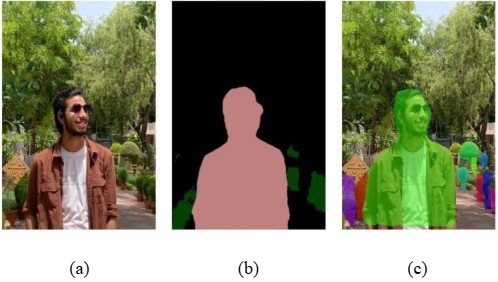
\includegraphics[width=10cm]{./assets/segmentation.jpg}
    \caption{Image Segmentation Explained from 
    \href{https://builtin.com/sites/www.builtin.com/files/styles/ckeditor_optimize/public/inline-images/1_image-segmentation\%202.jpeg}{Builtin.com}.}
    \label{fig:figure-2.1}  
\end{figure}

\begin{enumerate}
    \item[(a)] Original image
    \item[(b)] Semantic Segmentation
    \item[(c)] Instance Segmentation
\end{enumerate}

\subsubsection{Feature Extraction} Once the image has been segmented, the next step is to extract  features that can be used for further analysis, such as character recognition or form field identification. Feature extraction techniques identify important attributes such as: 

\begin{enumerate}
	\item \textbf{Color Image Processing:} Color image processing is classified into two types:
	\begin{enumerate}
		\item \textbf{Full-color processing:}involves images captured using full-color sensors, further divided into:
			\begin{enumerate}
			    	\item Individual Component Processing: Each color component (like RGB) is processed separately before creating a composite image.
			    	\item Direct Color Pixel Manipulation: Color pixels are manipulated directly.
			\end{enumerate}
	    	\item \textbf{Pseudo-color processing:} assigns colors to specific gray values based on criteria, utilizing techniques like intensity slicing and color coding.
	\end{enumerate}
	\item \textbf{Image Compression:} Image compression reduces the amount of information needed to represent a digital image, primarily to save storage space or reduce bandwidth during transmission. It is categorized into two types:
	\begin{enumerate}
	    	\item \textbf{Lossless Compression:} No information is lost during compression.
	    	\item \textbf{Lossy Compression:} Accepts some loss of information for higher compression rates.
	\end{enumerate}
	\item \textbf{Morphological Image Processing:} This technique focuses on extracting and analyzing the shape and structure of objects within an image. Common morphological operators include:
	\begin{enumerate}
		\item Boundary extraction
		\item Region filling
		\item Skeletonization
		\item Extraction of connected components
	\end{enumerate}
	\item \textbf{Representation and Description:} Post-segmentation, raw pixel data needs to be compacted for further analysis. Representation techniques can focus on external features (like boundaries) or internal features (like pixels covering the region). Common methods include:
	\begin{enumerate}
		\item \textbf{Chain Codes and Polygonal Approximations:} representing shapes.
		\item \textbf{Boundary Descriptors:} Include features like length, diameter, and curvature.
		\item \textbf{Regional Descriptors:} Describe image regions in terms of area, compactness, gray level statistics, and topological features.
	\end{enumerate}
\end{enumerate}

\subsubsection{Object Recognition} Object recognition is the process of identifying and classifying different regions in an image, referred to as patterns or objects. There are two main approaches to object recognition

\begin{enumerate}
	\item \textbf{Decision-Theoretic Approach:} This method uses numerical descriptions to analyze patterns. It looks at measurable features.
	\item \textbf{Structural Approach:} This approach focuses on qualitative descriptions, using relational descriptors that describe the relationships and arrangements between different parts of the patterns.
\end{enumerate}
 
\subsection{Optical Character Recognition (OCR)} OCR or Optical Character Recognition is an input device used to read a printed text. OCR scans text in image, analyzes it character by character and converts it into machine-readable code and stores text on the system memory and processes it as a document. OCR is widely used in applications where transforming printed material into editable text.

\subsubsection{OCR Architecture} After \textbf{image processing}, OCR comes into play. It extracts the text from the processed images, analyzing the document character by character to convert it into machine-readable code. It converts printed or handwritten text from forms into digital text, which can then be manipulated and stored. Once OCR extracts the raw text, \textbf{text processing} helps clean, format, and analyze this text.

\begin{figure}[H]
\centering
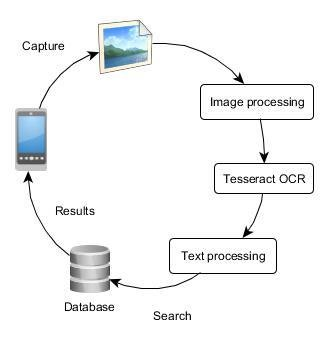
\includegraphics[width=10cm]{./assets/OCR-Process.png}
\caption{OCR Process}
\caption{OCR Process from 
\href{https://www.researchgate.net/profile/Adrian-Gomez-9/publication/281099638/figure/fig4/AS:614266293997575@1523463905255/Architecture-diagram-for-the-OCR-alternative.png}{Researchgate.net}.}
\label{fig:figure-2.2}
\end{figure}

\subsubsection{Post OCR error correction} After Extract the text from the image, The OCR are required a post OCR error correction because the text that the OCR have extracted may not misspelling and character miss order and the post OCR have following approach.

\begin{enumerate}
	\item \textbf{Symmetric Delete Spelling Correction:} Symmetric Delete Spelling Correction is works by generating possible corrections for misspelled words using a deletion-based algorithm. First, a precomputed dictionary is built by selecting valid words and generating variations with up to N deleted characters. These variations function as keys, leading back to the correct words. When a user types a misspelled word, the algorithm generates similar deletions and looks for matches in the precomputed dictionary. If a match is found, the appropriate word is suggested.
	
	\item \textbf{TF-IDF and Cosine Similarity:} TF-IDF is a technique that use to change a word into number or vector and the cosine similarity is a technique that use to measure how similar between two documents, and we will use a dictionary and convert it into vector, then compare with error word and find the closest distance.
	
\[
\text{TF-IDF}(t, d) = \text{TF}(t, d) \times \text{IDF}(t)
\] \\
	
\[
\text{Cosine Similarity} = \frac{\sum_{i=1}^{n} A_i B_i}{\sqrt{\sum_{i=1}^{n} A_i^2} \times \sqrt{\sum_{i=1}^{n} B_i^2}}
\]

\end{enumerate}

\subsection{Natural Language Processing (NLP)} Natural Language Processing (NLP) enables machines to understand, interpret, and generate human language in a valuable way. The process involves several key techniques: Tokenization: Breaking down text into smaller units (tokens), such as words or phrases, which can be analyzed separately. Stop Word Removal: Eliminates common words that provide little informational value, focusing on more meaningful words. Lemmatization and Stemming: Reduces words to their root forms to unify different inflected versions (e.g., "walking" becomes "walk"). Part-of-Speech Tagging: Assigns tags to words based on their grammatical roles (nouns, verbs, adjectives, etc.).

\subsection{Deep Learning} Deep Learning is a type of machine learning where computers are trained to think and learn like humans by processing large amounts of data. It uses a special kind of program called a neural network, which is inspired by the way our brains work. These networks can figure out patterns and make decisions on their own, such as recognizing faces in photos, translating languages, or even predicting what you might want to buy.

\begin{figure}[H]
\centering
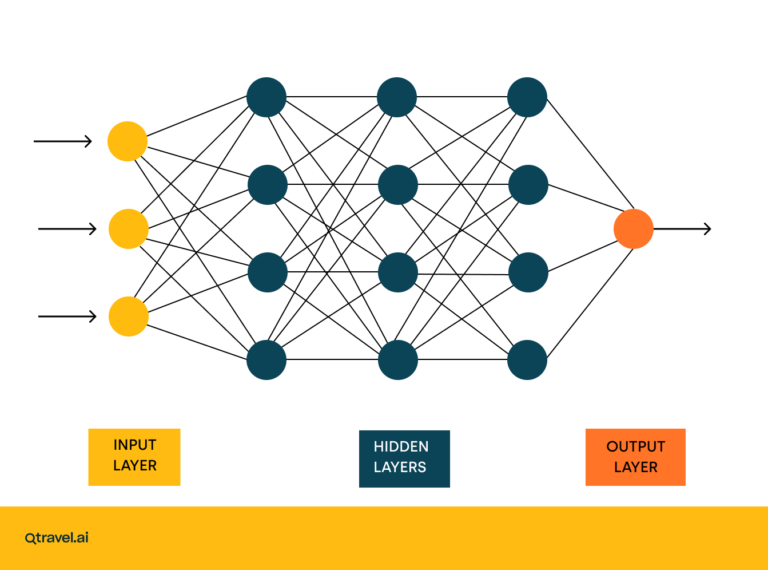
\includegraphics[width=10cm]{./assets/Natural-Network.png}
\label{fig:figure-2.3}
\caption{Natural Network from 
\href{https://www.qtravel.ai/wp-content/uploads/2023/07/sieci-neuronowe-grafika-768x570.png}{Qtravel.ai}.}
\end{figure}

\subsection{Generative AI} Generative AI refers to deep learning models that can generate high-quality text, images, and other content based on trained data.  It works by analyzing a lot of data, such as Wikipedia articles or famous paintings, and then using what it learns to produce original outputs similar to the data it studied. \par
In the past, AI models like Variational Autoencoders (VAEs) and Generative Adversarial Networks (GANs) helped create realistic images and sounds. Now, newer models like transformers have taken over. Transformers are powerful because they can learn from massive amounts of text without needing people to label everything.

\subsubsection{Types of Transformer models}
\begin{enumerate}
	\item \textbf{Encoder-only models} (such as BERT): Great for understanding and categorizing text but not for generating new content.
	\item \textbf{Decoder-only models} (such as GPT): Focus on predicting the next word and are good at creating new text.
	\item \textbf{Encoder-decoder models} (such as T5): Combine both approaches and can handle tasks like summarizing or translating text.
\end{enumerate}

\subsection{Security of Web Form} Web form security is essential as these forms are highly vulnerable to cyberattacks, making them prime targets for malicious parties aiming to access sensitive user data. 
Common threats include:
\begin{enumerate}
	\item \textbf{Cross-Site Scripting (XSS):} Attackers inject malicious scripts into web forms or application code, which can steal user information like keystrokes or cookies, or redirect users to harmful websites.
	\item \textbf{SQL Injection:} Attackers manipulate SQL code within web forms to access or alter databases. This technique can expose or modify sensitive data, and it’s one of the oldest and most dangerous web vulnerabilities.
	\item \textbf{Cross-Site Request Forgery (CSRF):} Attackers trick users into performing unintended actions, such as submitting forms or transferring data, without their knowledge. These attacks exploit the user’s browser and session data.
	\item \textbf{Data Breaches:} A variety of attacks can lead to breaches, exposing sensitive customer information and damaging a business's reputation, as users lose trust in the website's security.
\end{enumerate}

	Many data privacy laws now regulate how web applications must ensure security, especially when handling personal information. The rules we must follow may depend on where our business is located and how it operates. To stay compliant, website owners need to adopt secure practices for web forms.

\textbf{Key laws to be aware of}
\begin{enumerate}
	\item \textbf{GDPR (General Data Protection Regulation)}
	\item \textbf{CCPA, CPRA (California Consumer Privacy Act and California Privacy Rights Act)}
	\item \textbf{HIPAA (Health Insurance Portability and Accountability Act)}
	\item \textbf{PCI DSS (Payment Card Industry Data Security Standard)}
\end{enumerate}

\textbf{Key measures for securing web forms}
\begin{enumerate}
	\item \textbf{Use TLS/SSL Certificates:} TLS/SSL certificates create encrypted links between browsers and servers, ensuring that data transferred is protected. Extended Validation (EV) certificates provide the highest level of security.
	\item \textbf{Encrypt Data:} End-to-end encryption (E2EE) ensures that data is protected throughout its journey from sender to recipient, preventing unauthorized access. Use SSL certificates and CDNs to enhance security.
	\item \textbf{Validate and Sanitize Input:} Validate and sanitize user inputs to prevent attacks like SQL injections or cross-site scripting (XSS). Validation checks if inputs are correct, while sanitization removes harmful data.
	\item \textbf{Collect Minimal Data:} Only collect necessary information to reduce the impact of potential data breaches. This minimizes risk and aligns with privacy regulations like GDPR and CCPA.
	\item \textbf{Anonymize Data:} Mask sensitive data (e.g., credit card numbers) using techniques like asterisks or data shuffling, making it harder for attackers to misuse it.
	\item \textbf{Ask for Consent:} Obtain clear user consent before collecting personal data, and provide easy access to your privacy policy outlining how data is used and protected.
	\item \textbf{Restrict File Uploads:} Limit file uploads by allowing only authorized users, setting file size limits, and using whitelist file types to prevent malware.
	\item \textbf{Use reCAPTCHA:} Implement reCAPTCHA to differentiate between humans and bots, helping reduce spam and prevent automated attacks.
	\item \textbf{Require Authentication:} For sensitive forms, require users to authenticate (e.g., through login or multi-factor authentication) to restrict access to authorized individuals only.
	\item \textbf{Use Virus and Malware Protection:} Employ virus and malware protection through layered security, such as firewalls, malware scans, and intrusion detection, to safeguard your web forms from threats.
\end{enumerate}

\section{Languages and technologies}
\subsection{Web Development Language}
\subsubsection{HTML} HTML (HyperText Markup Language) is the standard language for creating and designing web pages. It is a markup language, which means that specific tags are used to structure web content. Each tag specifies a particular aspect of a website, such as text, photos, links, and multimedia.

\subsubsection{TypeScript} TypeScript is a superset of JavaScript that introduces static typing. It was created by Microsoft to solve some of the limitations of JavaScript, particularly in large-scale applications. Because TypeScript is a superset, it supports all JavaScript features while also adding new functionalities, notably those aimed at increasing code dependability and maintenance.

\subsection{Front-end Technology}
\subsubsection{Vue.js} Vue.js is a JavaScript framework for building user interfaces. It builds on top of standard HTML, CSS, and JavaScript and provides a declarative, component-based programming model that helps you efficiently develop user interfaces of any complexity.

\subsubsection{TailwindCSS} Tailwind CSS is a utility-focused CSS framework that simplifies web development by providing pre-designed utility classes. These utility classes allow you to create custom designs.

\subsubsection{SurveyJS} SurveyJS is a set of JavaScript components that allow users to build surveys, quizzes, polls, and other web forms, store them in your database, and visualize survey results in custom dashboards.

\subsection{Backend Technology}
\subsubsection{FastAPI} FastAPI is a modern web framework for creating Python APIs that prioritizes speed, ease of development, and automated validation. It has gained popularity for developing quick, high-performance APIs because it uses Python type hints to provide explicit, automatic data validation and interactive API documentation.

\subsubsection{Pydantic} Pydantic is a Python data validation and parsing library that enforces data types and restrictions using Python type annotations. Although it can be used separately, it is an essential part of FastAPI. With Pydantic models, you can easily serialize data, validate incoming data, and specify the structure of your data.

\subsubsection{SQLAlchemy} SQLAlchemy is the Python SQL toolkit and Object Relational Mapper that gives application developers the full power and flexibility of SQL without creating a SQL statement.

\subsubsection{PostgresSQL} The PostgreSQL popular open-source relational database management system (RDBMS) for managing and storing data. It is renowned for being reliable, effective, and compliant with SQL standards. And It support storing a json format data type which it can be act as NoSQL in some situation.

\subsection{Document Processing}
\subsubsection{Python} Python Programming language is a popular high-level computer programming language for machine learning because it is simple to use and easy to read and write. Additionally, it has a fast processing speed. Web development, data analysis, automation, scientific computing, and many more topics are among the many libraries available.

\subsubsection{Open Source Computer Vision Library (OpenCV)} Open Source Computer Vision Library is an open-source library designed for real-time computer vision and image processing. It provides tools for tasks such as object detection, image segmentation, facial recognition, and edge detection. OpenCV is widely used in fields like robotics, augmented reality, and machine learning.\par
OpenCV processes image data using built-in functions for manipulating pixel values. It works with image and video formats and can be integrated with machine learning models to perform visual recognition tasks. It supports various languages, including Python

\subsubsection{Tesseract OCR} Tesseract OCR is an open-source Optical Character Recognition (OCR) engine used to convert images of text into machine-encoded text. Developed by Hewlett-Packard and maintained by Google, it supports various languages and one of them is python, making it highly versatile for tasks like digitizing printed materials, extracting text from images, and enhancing accessibility in digital applications. It is commonly integrated with other image processing libraries like OpenCV to handle pre-processing tasks, improving text recognition accuracy, especially in noisy or distorted images.

\subsubsection{NLLB-200} NLLB-200 (No Language Left Behind) is a project by Meta (Facebook) that focuses on creating AI models capable of translating between 200 languages.

\subsubsection{PyTorch} PyTorch is an open-source deep learning framework developed by Facebook's AI Research lab (FAIR). It provides tools for building and training neural networks using dynamic computational graphs, which allow for flexibility and ease in model building.

\subsubsection{LLAMA} LLama (short for Large Language Model Architecture) is a type of AI model designed to understand and generate human-like text. It is built using a transformer architecture, which helps it learn language patterns and produce meaningful responses based on its training data.

\section{Competing solutions}
\subsection{Microsoft Azure Document Intelligence}
\begin{figure}[H]
\centering

\includegraphics[width=10cm]{./assets/Microsoft-Azure.jpg}
\caption{Microsoft Azure Document Intelligence from 
\href{https://learn.microsoft.com/th-th/training/achievements/extract-data-from-forms-use-form-recognizer.svg}{Learn.microsoft.com}.}
\label{fig:figure-2.4}  
\end{figure}

	Microsoft Azure Document Intelligence is a solution that provides a feature of  capturing data from printed or handwritten forms. And create a flow pipeline with Azure Cognitive Search pipeline to complete workflow as the user needs.
%%%%%%%%%%%%%%%%%%%%%%%%%%%%%%%%%%%%%%%%%%%%%%%%%%%%%55
%%%%%%%%%%%%%%%%%%%%%%%%%%%%%%%%%%%%%%%%%%%%%%%%%%%%%
%%%%%%%%%%%%%%CHAPTER 3 DESIGN AND METHODOLOGY%%%%%%%%%%%%%%%%
%%%%%%%%%%%%%%%%%%%%%%%%%%%%%%%%%%%%%%%%%%%%%%%%%%%%%
\chapter{DESIGN AND METHODOLOGY}

This chapter will cover the features, architecture, functionalities, design methods, and
diagrams of our web application. We will delve into the details of the application’s
functionality and architecture.

\section{Project Functionality}

\subsection{System Requirements}

\begin{itemize}
 \item The web application must allow users to log in with email and password. 
 \item The web application must allow the user to upload a form file to the system.
 \item The web application must allow users to fill the form without login.
 \item The web application must allow users to view the data of the form.
 \item The web application must allow users to edit the form before publishing.
 \item The web application must allow users to delete the form.
 \item The web applications must provide the option for all logged-in users to logout.
\end{itemize}

\subsection{Feature List}

\subsubsection{Paper-Based Form Analysis System}

The Paper-Based Form Analysis System will extract all the text from the document that is uploaded by the user via a web application. The system will then analyze the form’s pattern ,extract the input labels, translate the text into English, and send the translated information to a generative AI for data type generation.

\subsubsection{Form Schema generator System}

The Form Schema generator System will receive information from the Paper-Based Form Analysis System and Form Schema generator System must be able to generate a form schema that compatible with a form library.

\subsubsection{Web Form System}

The Web Form System must enable users to complete the form, store the data in the database, and see the data created by the form owner.

\subsubsection{Registration and Authentication System}

The Registration and Authentication System must enable a user to register and login to the system by using only email and password. This including a forgot password and the  OTP for reset password.	


\section{Use Case Diagram}

From the figure \ref{fig:use-case} The diagram shows a relationship between the user and the system by using a use case diagram. The user of the system is a developer that needs to transform a paper-base form into web application form and the user who going to fill the form. The system consists of 3 different systems, which are paper-based form analysis systems, form schema generator systems, web form systems and registration and authentication systems. The user can upload a paper-based form to the system, and the system will transform the form into a web-based form.

\begin{figure}[!h]
\centering
\fbox{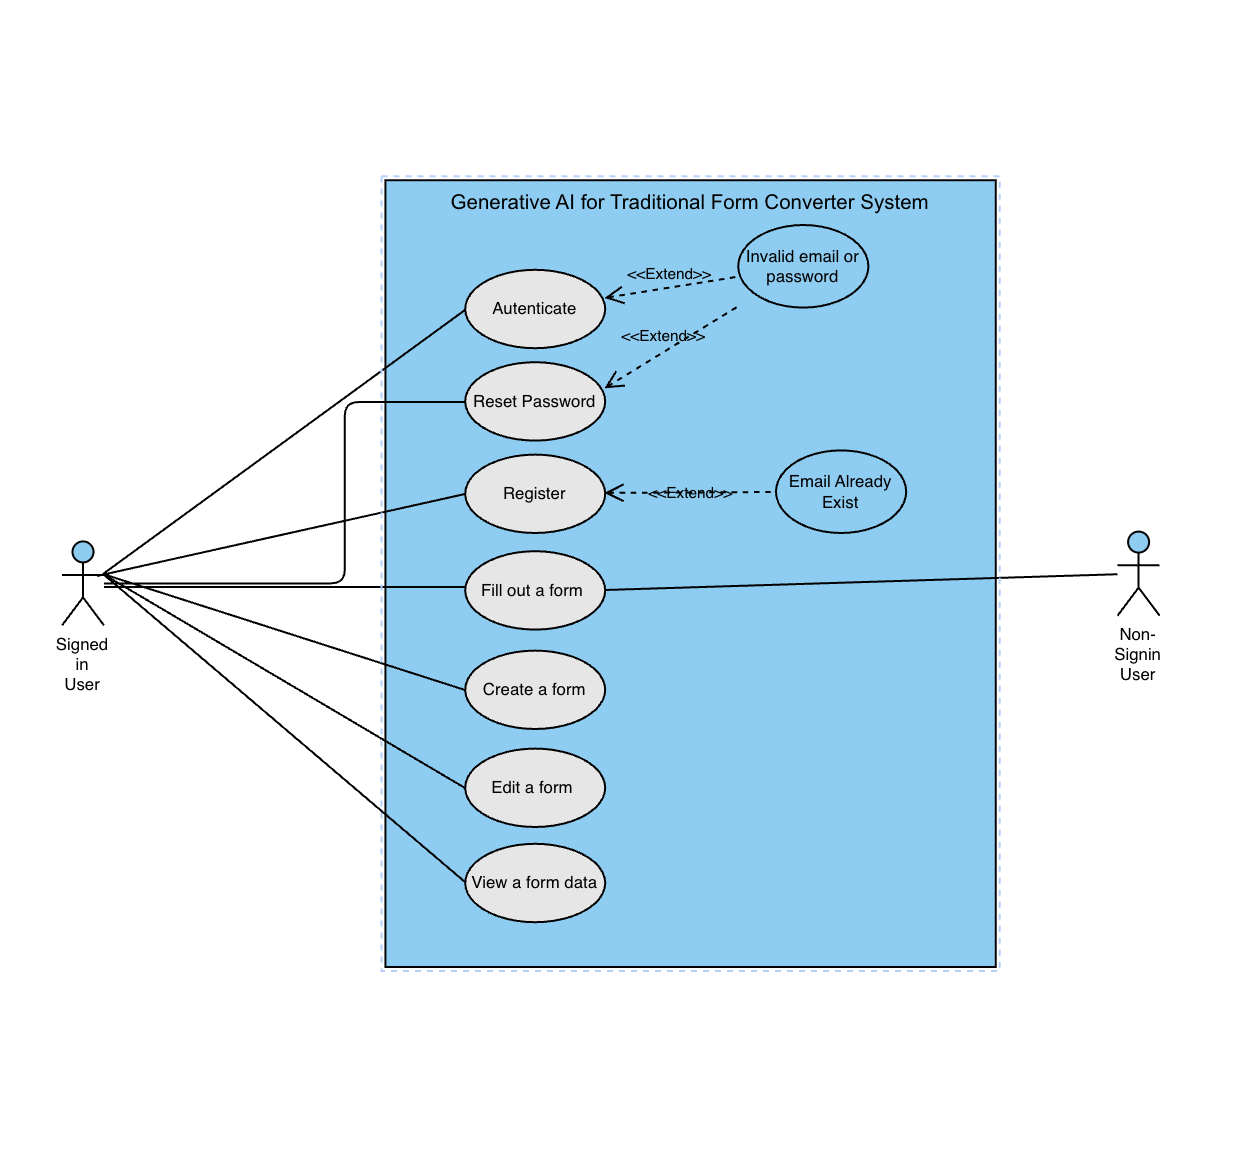
\includegraphics[width=10cm]{./assets/usecase.png}}
\caption{Use case diagram}\label{fig:use-case}
\end{figure}

\section{Use Case Narrative}

\subsection{Autentication}

\textbf{Use Case Name:} Autentication \\
\textbf{Actors:} Form Creator and Required Login User \\
\textbf{Goal:} Users log in to the system. \\
\textbf{Preconditions:} User is registered

Main Success Scenario: 

\begin{enumerate}
    \item User access the website.
    \item User enter a email and password.
    \item User submit a email and password.
    \item System authenticate and navigate to the home page.
\end{enumerate}

\subsection{Register}

\textbf{Use Case Name:} Register \\
\textbf{Actors:} Form Creator and Required Login User \\
\textbf{Goal:} Users register to a system. \\
\textbf{Preconditions:} User does not have an account

Main Success Scenario: 

\begin{enumerate}
    \item User access the website.
    \item User click to create a new account.
    \item User enter an email and password and personal information.
    \item User submit information.
    \item System saves user information and navigates users to the login page.

\end{enumerate}

\subsection{Create a form}

\textbf{Use Case Name:} Create a form \\
\textbf{Actors:} Form Creator\\
\textbf{Goal:} Create a form by upload the form file. \\
\textbf{Preconditions:} User has logged in.

Main Success Scenario: 

\begin{enumerate}
    \item User go to home page.
    \item User click at upload a form.
    \item User select a file to upload.
    \item System will process the file and navigate users to the edit form page to confirm a form before publishing.
   
\end{enumerate}

\subsection{Edit a form}

\textbf{Use Case Name:} Edit a form \\
\textbf{Actors:} Form Creator\\
\textbf{Goal:} Edit a form to make a change.\\
\textbf{Preconditions:} User has logged in.

Main Success Scenario: 

\begin{enumerate}
    \item User go to home page.
    \item User click at edit a form at the form user need to make change.
    \item User make change a form.
    \item User click back to the previous page.
    \item System will process autosave and navigate users to the previous page.
\end{enumerate}


\subsection{View a form data}

\textbf{Use Case Name:} View a form data \\
\textbf{Actors:} Form Creator\\
\textbf{Goal:}View the data that user have input\\
\textbf{Preconditions:} User has logged in.

Main Success Scenario: 

\begin{enumerate}
    \item User go to home page.
    \item User click at view a data of the form.
    \item User can see a form data
\end{enumerate}

\subsection{Fill up the form}

\textbf{Use Case Name:} Fill up the form \\
\textbf{Actors:} Required Login Users and Anonymous User \\
\textbf{Goal:} Add a new data to the form \\
\textbf{Preconditions:} User has logged in or non-login user.

Main Success Scenario: 

\begin{enumerate}
    \item User access a form via the public link
    \item User fill up a form.
    \item User submit a form data.
    \item System will save the data and navigate to the form page again.
\end{enumerate}

Alternate scenario (user access the form required a login without login):

\begin{enumerate}
    \item User access a form via the public link
    \item System will navigate to the login page After login completes the user will redirect back to the form page.
\end{enumerate}


\section{Activity Diagram}

From Figure \ref{fig:activity-diagram} The Activity diagram shows the sequence how Generative AI for
Traditional Form Converter System is working.

\begin{figure}[!h]
\centering
\fbox{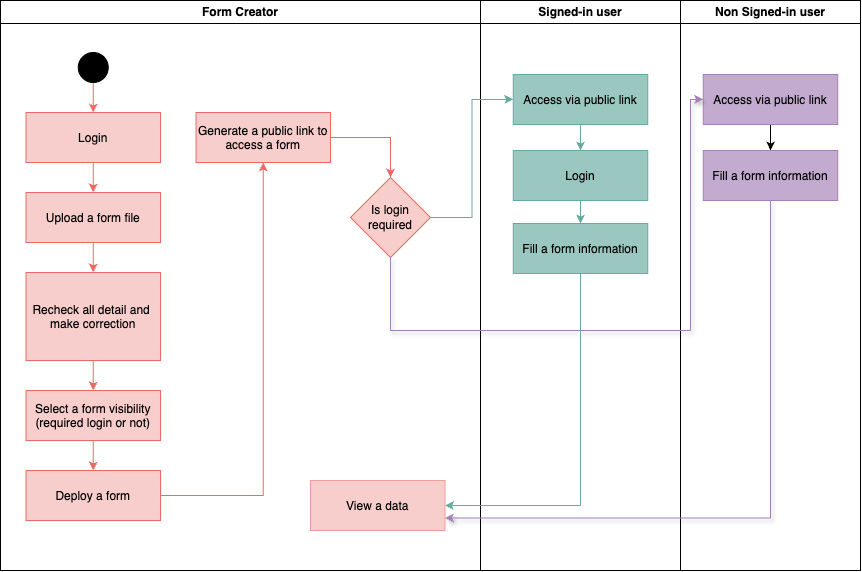
\includegraphics[width=10cm]{./assets/activity-diagram.png}}
\caption{Activity Diagram}\label{fig:activity-diagram}
\end{figure}


\newpage
\subsection{Form creator}

\begin{itemize}
\item  \textbf{Login:} Form Creator must login before use the system
\item  \textbf{Upload a form file:} After logging in, Form creator must upload a form file to add new form to the system.
\item  \textbf{Recheck all detail and make correction:} In this step, Form creator must check all the information that system has generated and make a correction if incase of error text found.
\item  \textbf{Select a from visibility:} Select a form visibility, whether the form creator need to form to be access by the user who signed-in or anyone can access.
\item  \textbf{Deploy a form and Generate a link:} In this step, the form will be saved and generated a link to allow user to access.

\end{itemize}


\subsection{Signed-in user}

\begin{itemize}
\item  \textbf{Login:} If the form requires login, the user must log into the system.
\item  \textbf{Fill out information:} Once logged in, the user going to fills out the form and submit.
\end{itemize}


\subsection{Non Signed-in user}

\begin{itemize}
\item  \textbf{Fill out information:} If login is not required, the user can directly fill out the form without logging in.
\end{itemize}


\section{System Architecture}

\begin{figure}[!h]
\centering
\fbox{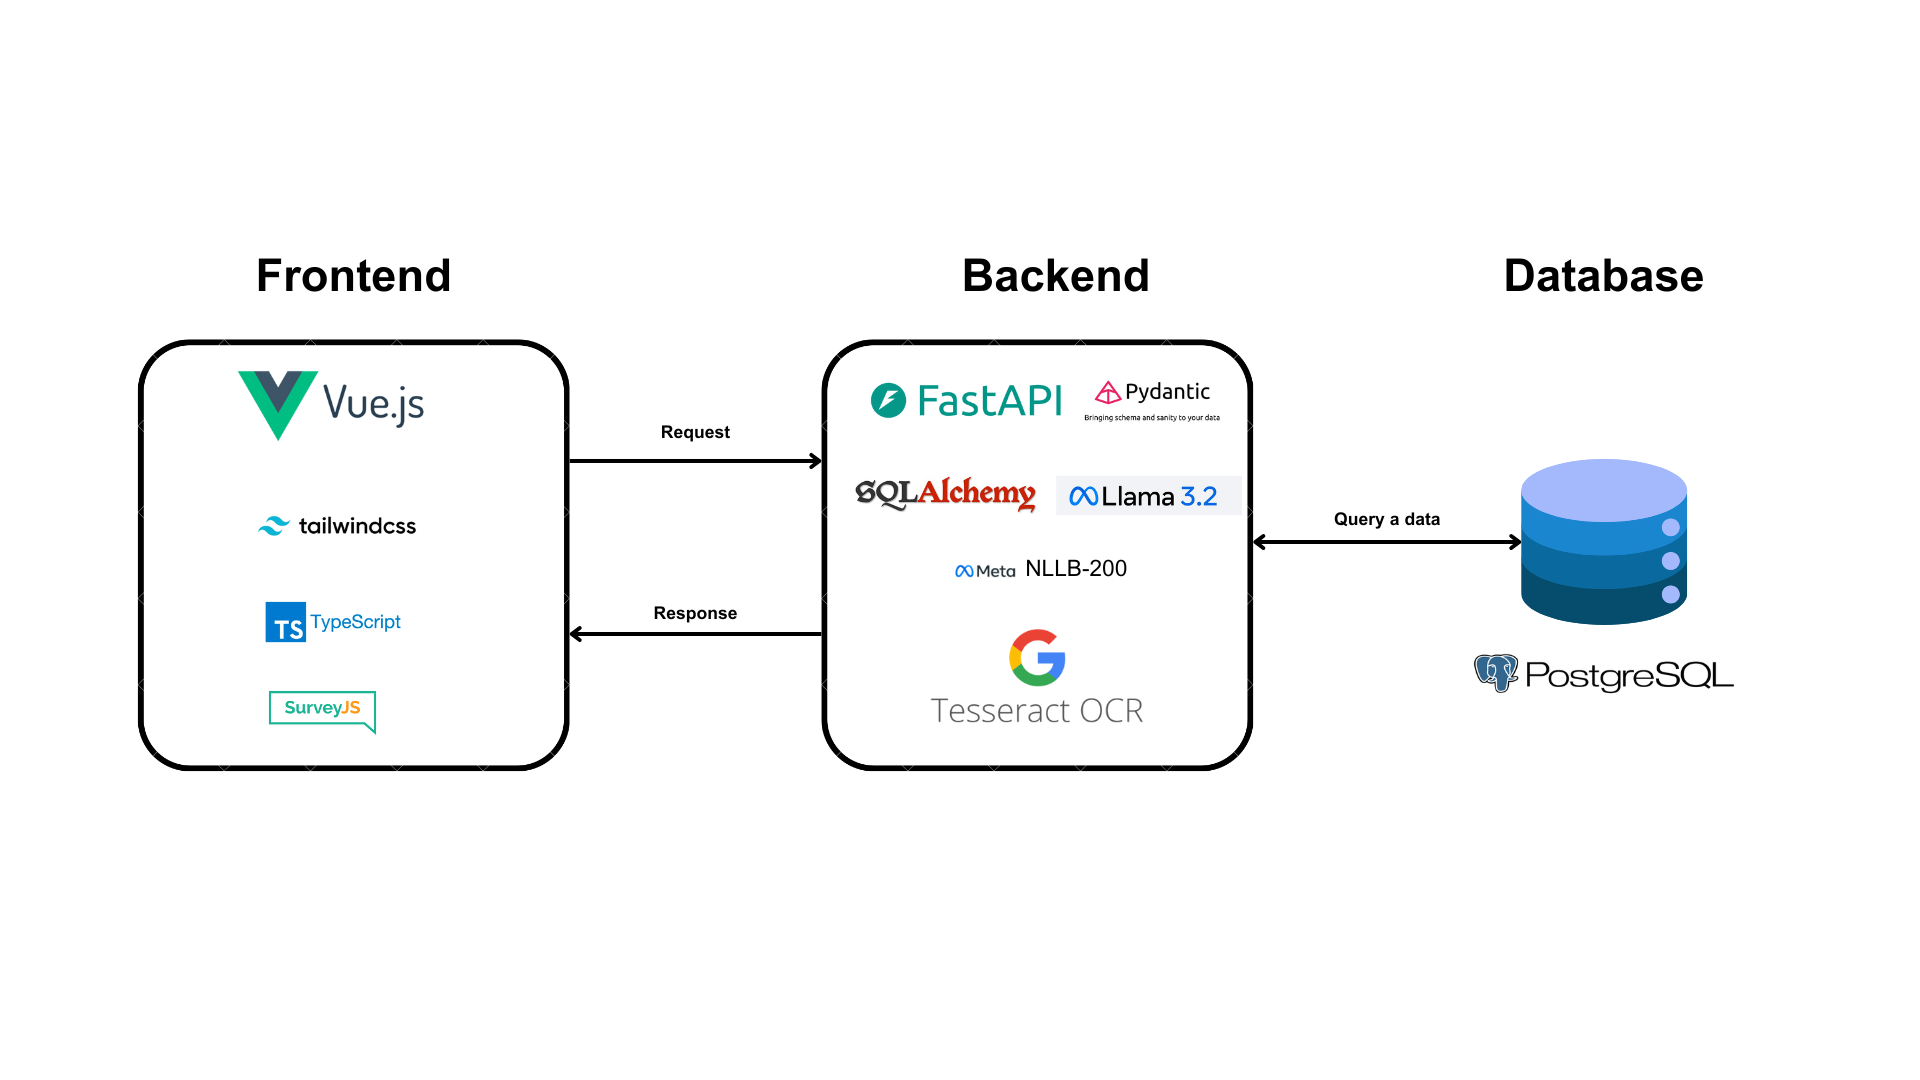
\includegraphics[width=10cm]{./assets/system-arch.png}}
\caption{System Architecture}\label{fig:system-arch}
\end{figure}

Figure \ref{fig:system-arch}, The diagram shown a system architecture in figure above, The System have divided into 3 part which front-end, back-end and database, each part have shown a technology stack, and here are the description of each component

\begin{itemize}
\item  \textbf{VueJS} is a Front-end JavaScript library for building UI
\item \textbf{TailwindCSS} is a CSS framework for styling the UI and used with React
\item \textbf{FastAPI} is a Back-end framework for building REST API
\item \textbf{PostgreSQL}  is a relational database
\item \textbf{Pydantic}  is a python library used for data validation 
\item \textbf{SQLAlchemy} is a Python base Object Relational Mapper (ORM) and SQL Tool kit
\item \textbf{SurveyJS} is a form engine Llibrary
\item \textbf{Meta NLLB-200} is a Model for text translation
\item \textbf{Tesseract OCR} is a OCR for extract text from image
\item \textbf{Llama 3.2} is a generative AI from Facebook
\end{itemize}


\section{System Worflow}

\subsection{Extracting text and text parse}

\subsubsection{Extracting text}

Extracting text is the first process after the user has uploaded a file via the web application, this step is going to extracting text from the file by using an OCR technique for images, but If the user has provided a PDF file, the system will use a PDF library, such as PyMuPDF or Pdfplumber to extract a text and the layout. The OCR technique requires additional steps because we must pre-process the image using a black-and-white scale, and enhance its quality and clarity before the OCR process can begin. A text will be returned by the system once the process is complete.

\subsubsection{Text Parse}

Text parsing is the second process after the extracted text has been completed. Text parse is the process of analyzing a text and breaking down the text to convert it into a structured format, In this process, the purpose of text parse is to analyze the layout of the form, by using a text from a previous process to identify where which text is the label of the input field. The text parse algorithm starts by separating the text from each line and analyzing it line by line, If there is a word in front of the small point the text parse will mark the text as an input label, but if the line starts with the small point the parse will look back to the previous line to check whether if there any text that matches with the condition that parse has.

\subsubsection{Text Error Correction}

Text Error Correction is the third process after extracting text and text parse, respectively. Text error correction is identifying and fixing errors in a given text. Text error correction includes spelling mistakes, grammatical errors, punctuation issues, and incorrect word usage. In this process, the text error correction focuses on spelling mistakes and vowel missed order, To make a correction, the first step is to tokenize the whole word into a single word and check the word with a dictionary, If the word does not exist then the system will mark it as an error like this "<ERROR>Wolrd</ERROR>". The system will correct the word with a cosine similarity technique, the technique will convert a dictionary into a vector and also an error text. It will rank with cosine similarity, then it will take the first rank to replace a text. This process is required only for the user who uploads an image.

\subsection{AI Model}

\subsubsection{Translation}

Translation is the fourth process and the first process that AI have involve in the project. Translation is the process of  translate a Thai text to English text by using No Language Left Behind (NLLB) from meta, which the model is aim for high-quality translations directly between 200 languages. And we have selected a fine-tuned version of NLLB, which is wtarit/nllb-600M-th-en model and use it via hugging face transformer.

\subsubsection{Data Type Generator}

The Data Type Generator is the fifth process after preparing the process before the data type generator. The Data type generator is designed to generate a suitable datatype of each input field, for example, birthdate must be Date instead of string, passport number must be string, or text instead of number. All of these types will be applied with the form schema to make a form able to validate a correct data input. The data type generator is going to use a Llama 3 for prompt and generate a schema, and it will use an ollama as an interface for connecting to and communicating with the Llama 3 local model.

\subsection{Form Schema Generator}

The Form Schema Generator is the last process of the flow, the form schema generator will be used to generate a form schema from the output received from the data type generator to show output on the webpage and interact with the user.

\begin{figure}[!h]
\centering
\fbox{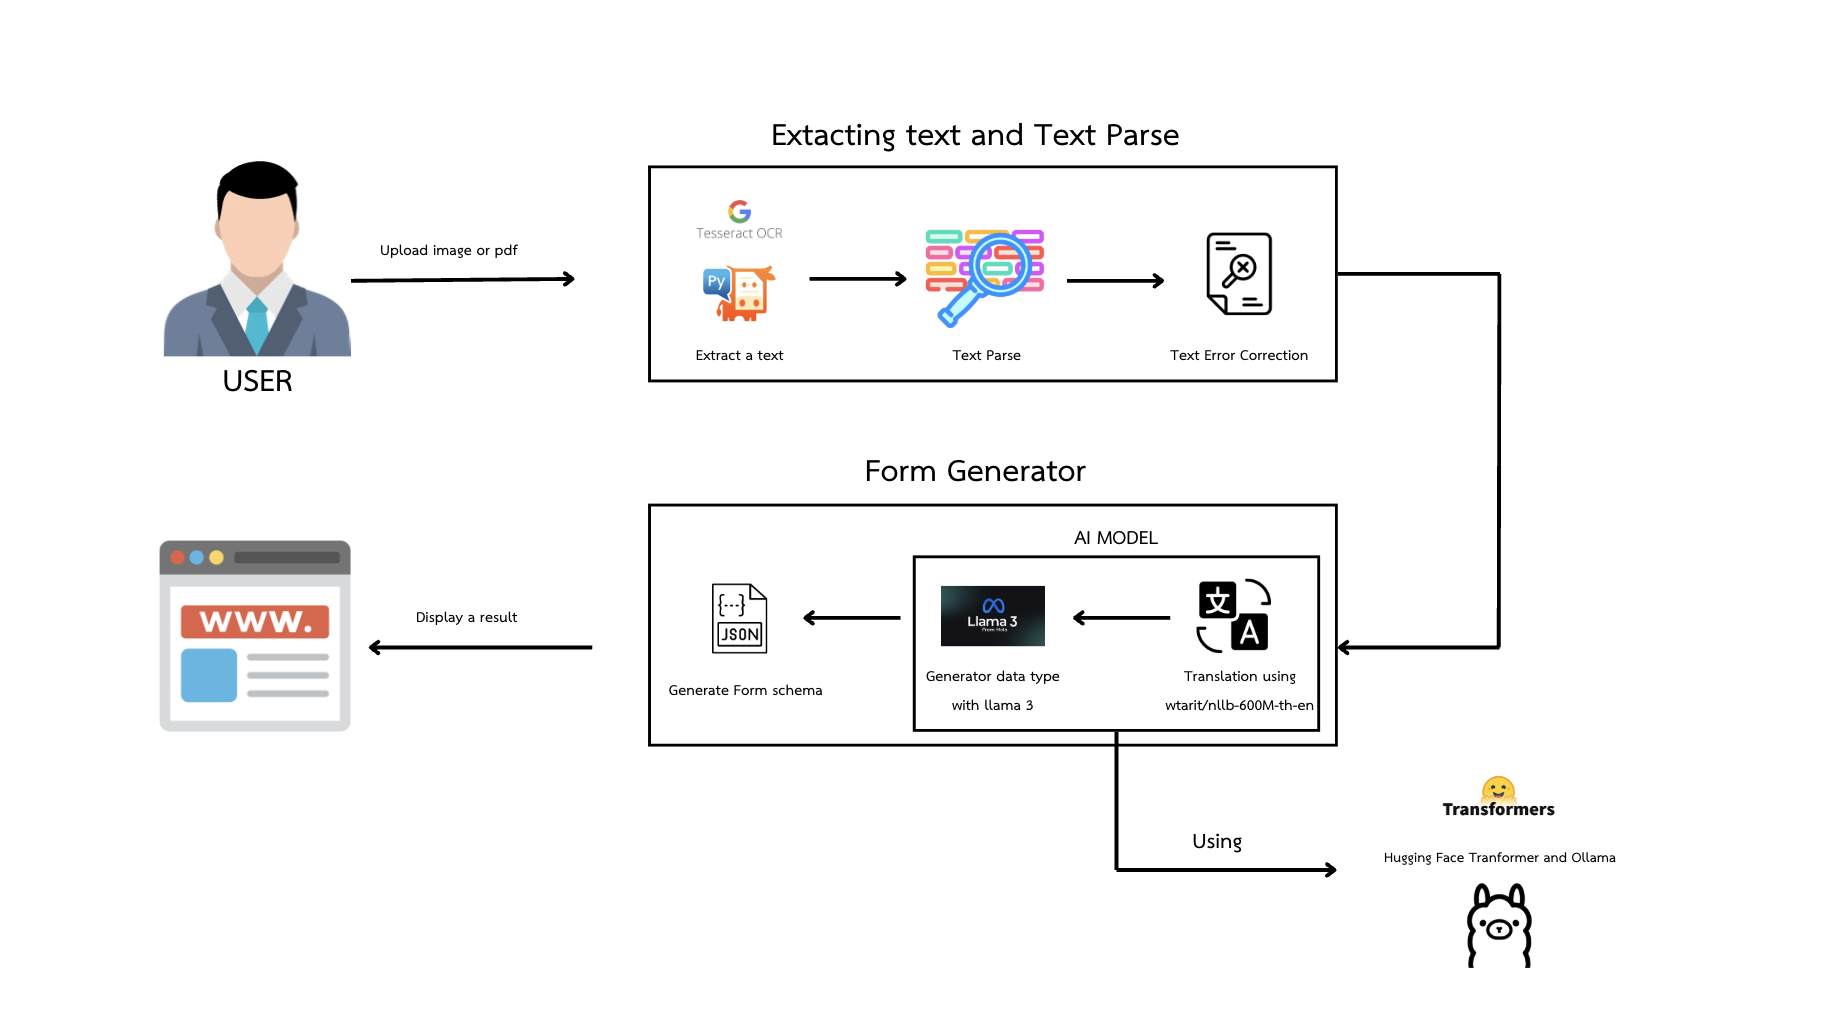
\includegraphics[width=10cm]{./assets/system-flow.png}}
\caption{System Workflow Diagram}\label{fig:system-workflow}
\end{figure}



\section{Database Design}

Figure \ref{fig:er-diagram} shown a project database design, the system consist three tables in our project database design are user, form, and form result. table is used to store user data, form result is used to store a result that the user has filled out, and form table is used to store a form schema.

\begin{figure}[!h]
\centering
\fbox{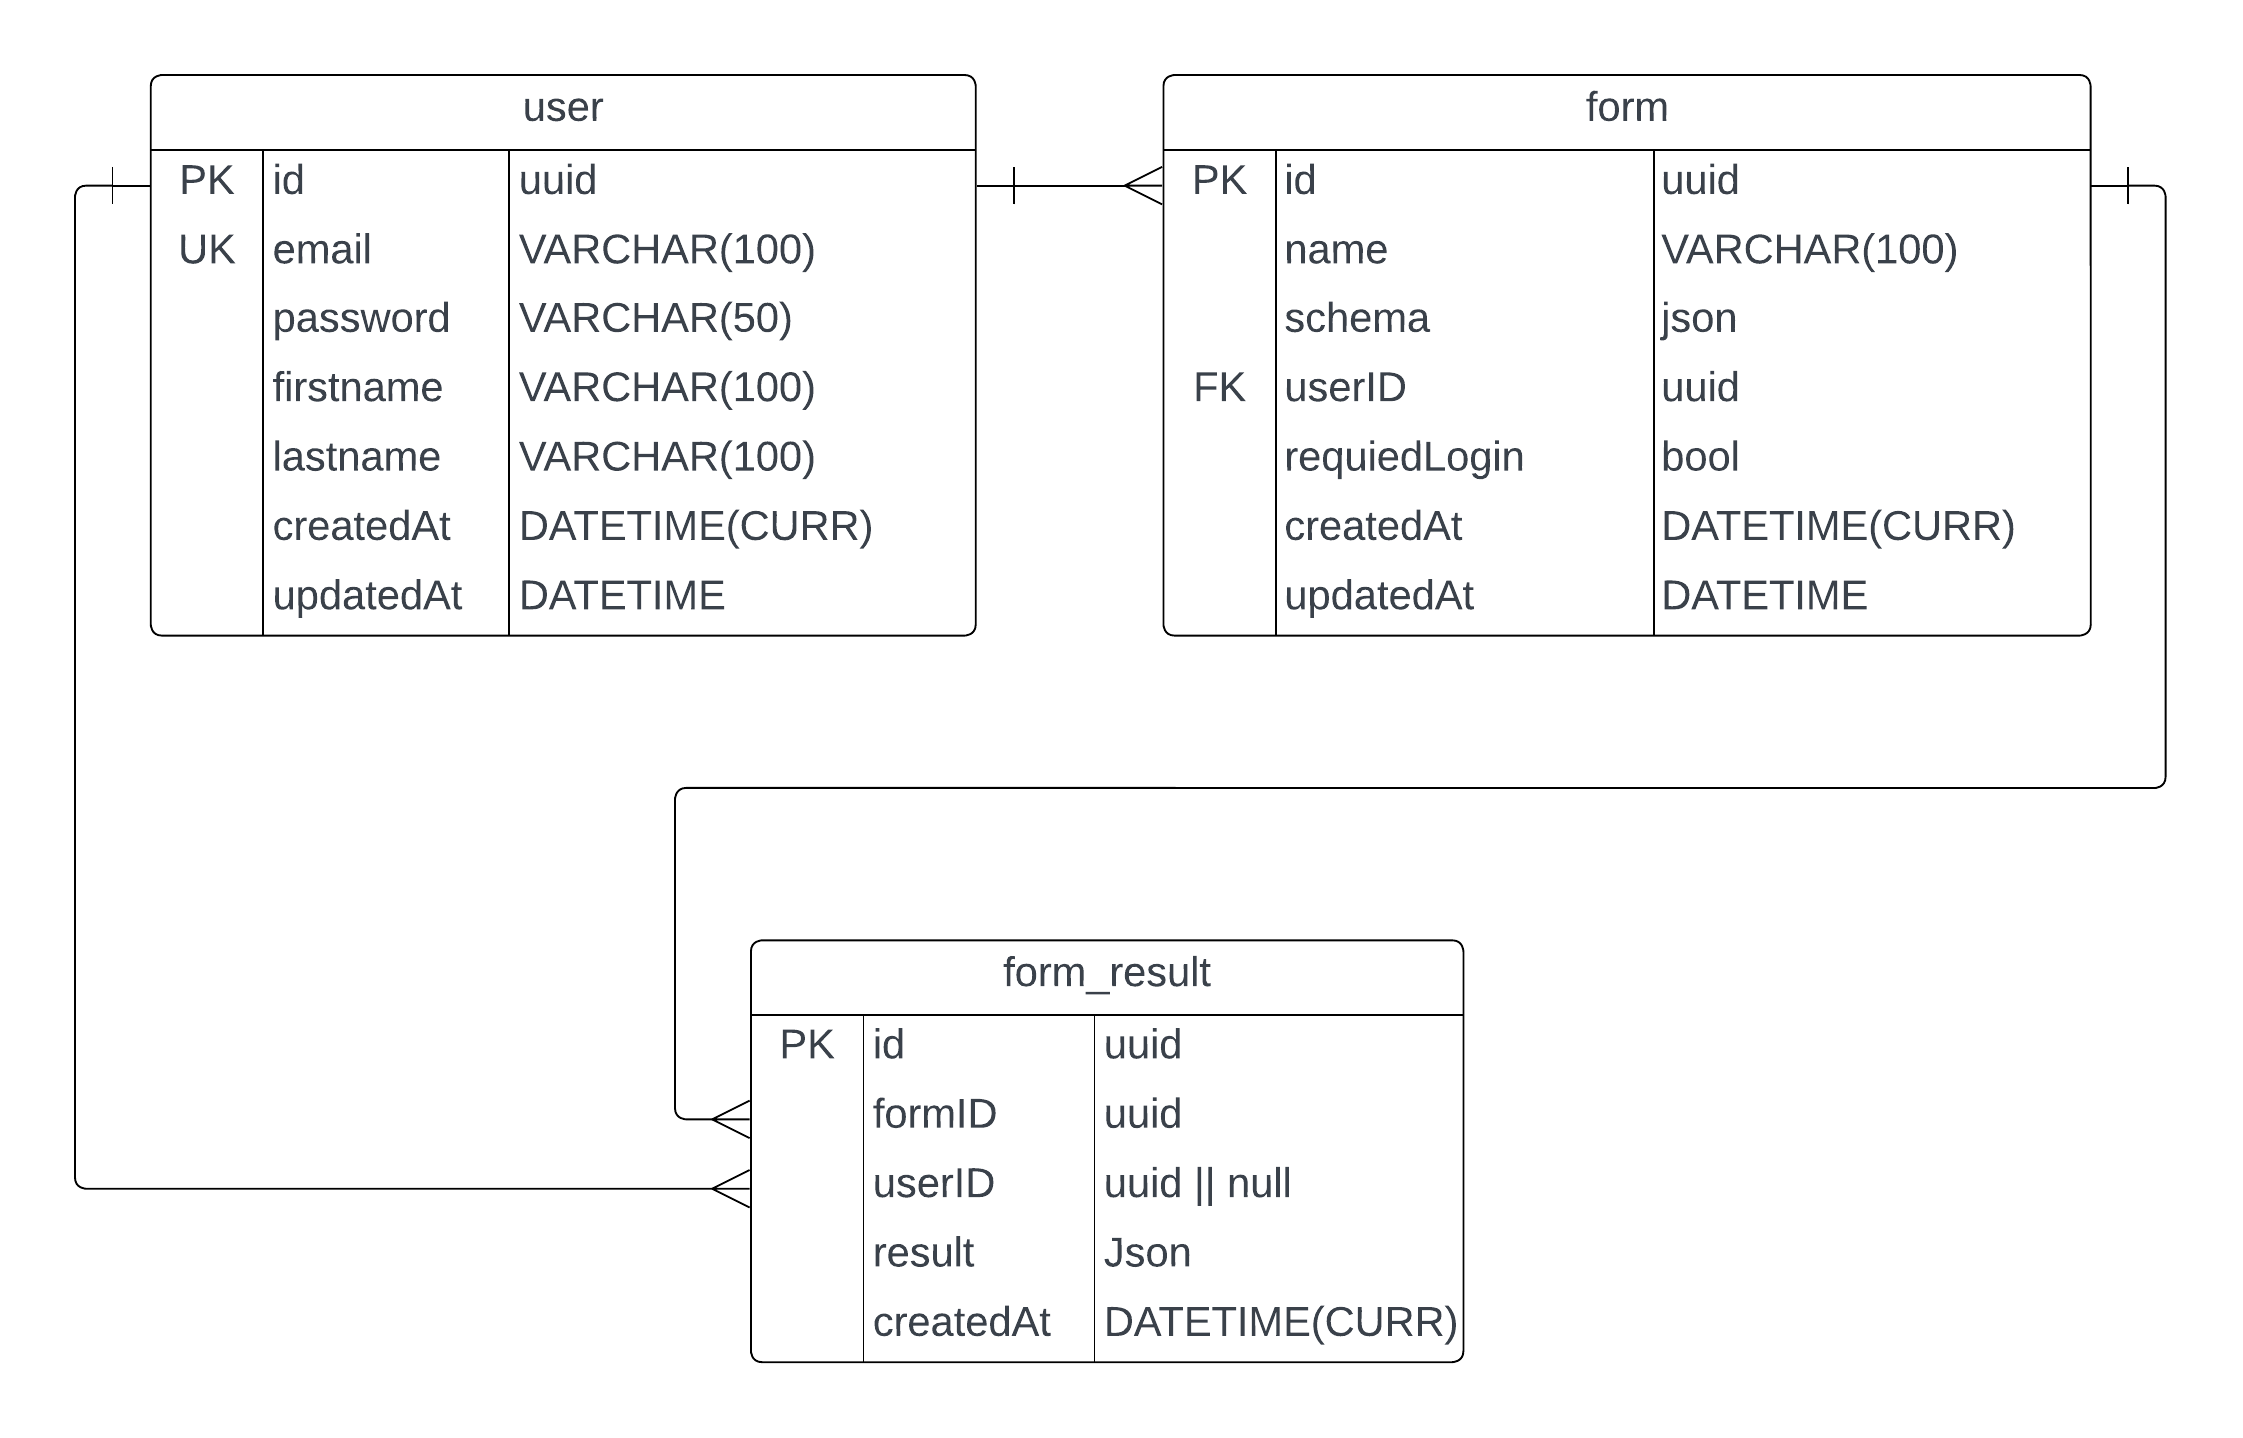
\includegraphics[width=10cm]{./assets/ER-diagram.png}}
\caption{ER Diagram}\label{fig:er-diagram}
\end{figure}


\newpage
\section{User Interface Design}

\subsection{Login Page}

\begin{figure}[!h]
\centering
\fbox{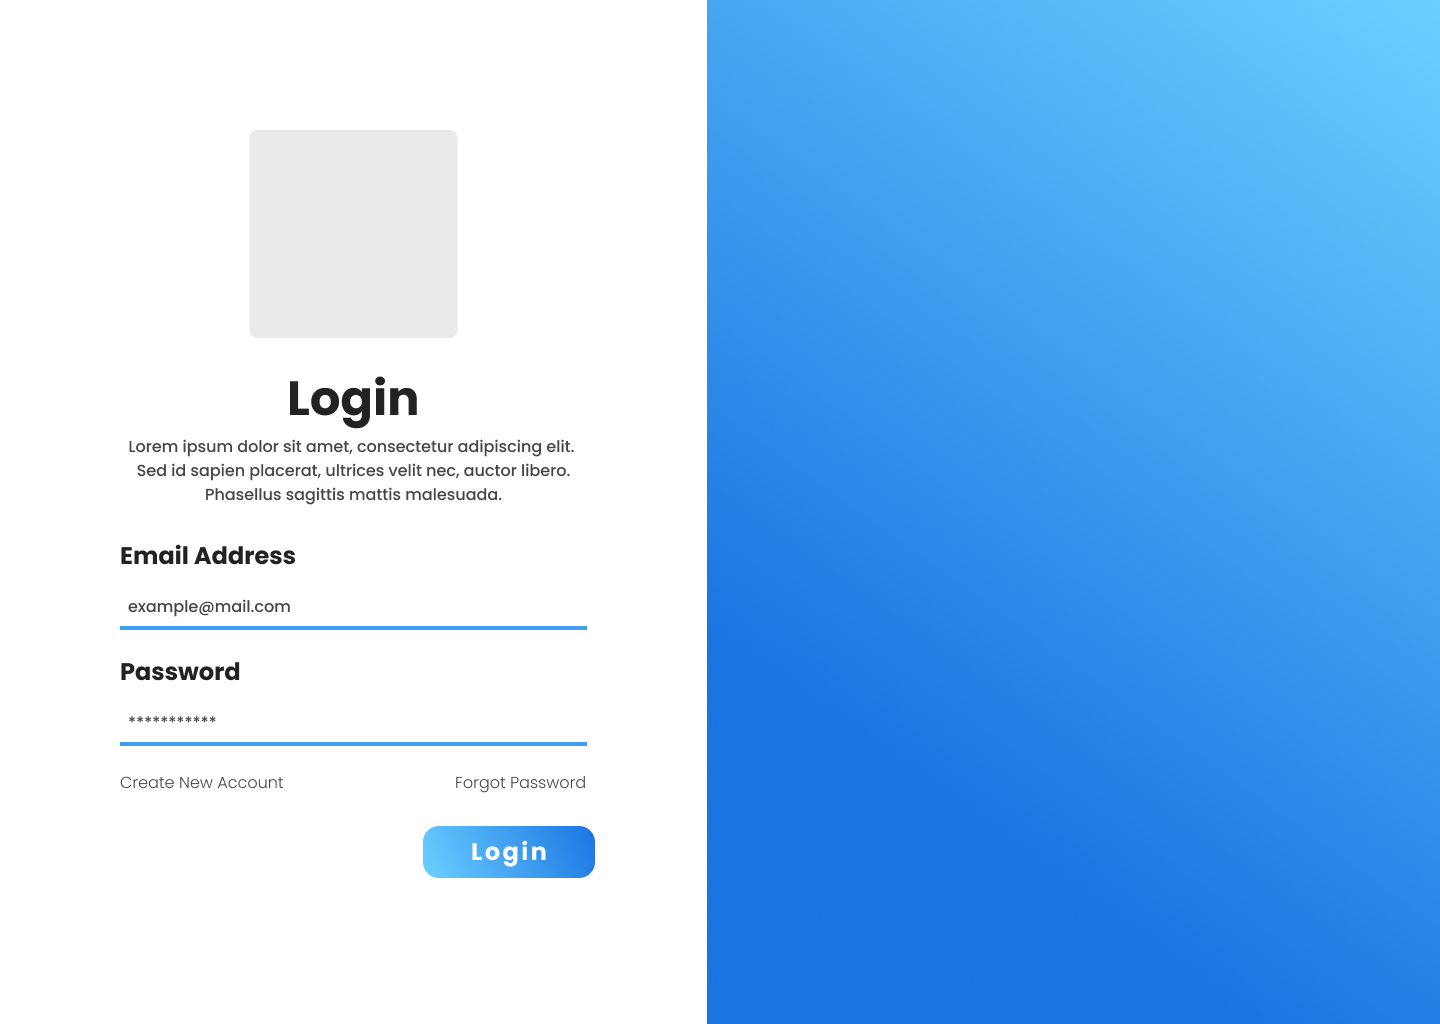
\includegraphics[width= 10cm]{./assets/UI/Login.png}}
\caption{Login Page}\label{fig:login}
\end{figure}

Figure \ref{fig:login} represents the login screen of the web application. This page have a email field,  password field and a login button to sent a credential to the back-end system. 

\subsection{Create Your Account }

\begin{figure}[!h]
\centering
\fbox{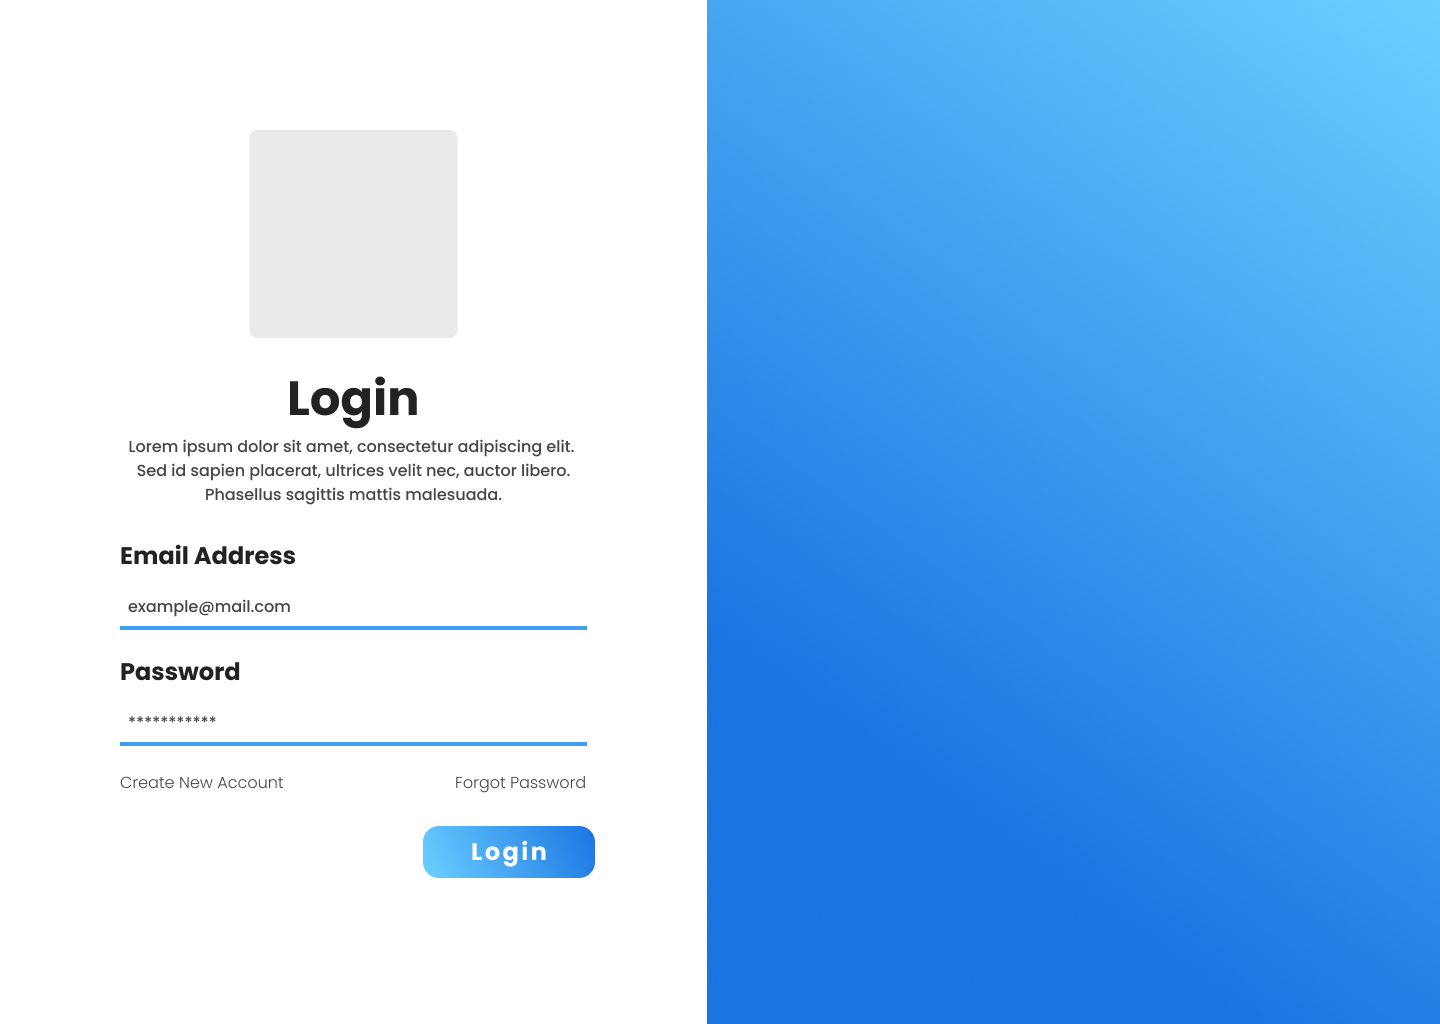
\includegraphics[width= 10cm]{./assets/UI/Login.png}}
\caption{Create Account Page}\label{fig:create-acc}
\end{figure}

Figure \ref{fig:create-acc} represents the create account page of the web application. This page allow user to create their own account by the user must provide a following field which is name, email and password.

\subsection{Forgot Password}

At Figure \ref{fig:Forgot-Password} represents the create account page of the web application. When the user forgot their password, The user must navigate to this page by click at forget password from login page. And fill the email address to allow the system sent the One-time password (OTP) to email address. 


\begin{figure}[!h]
\centering
\fbox{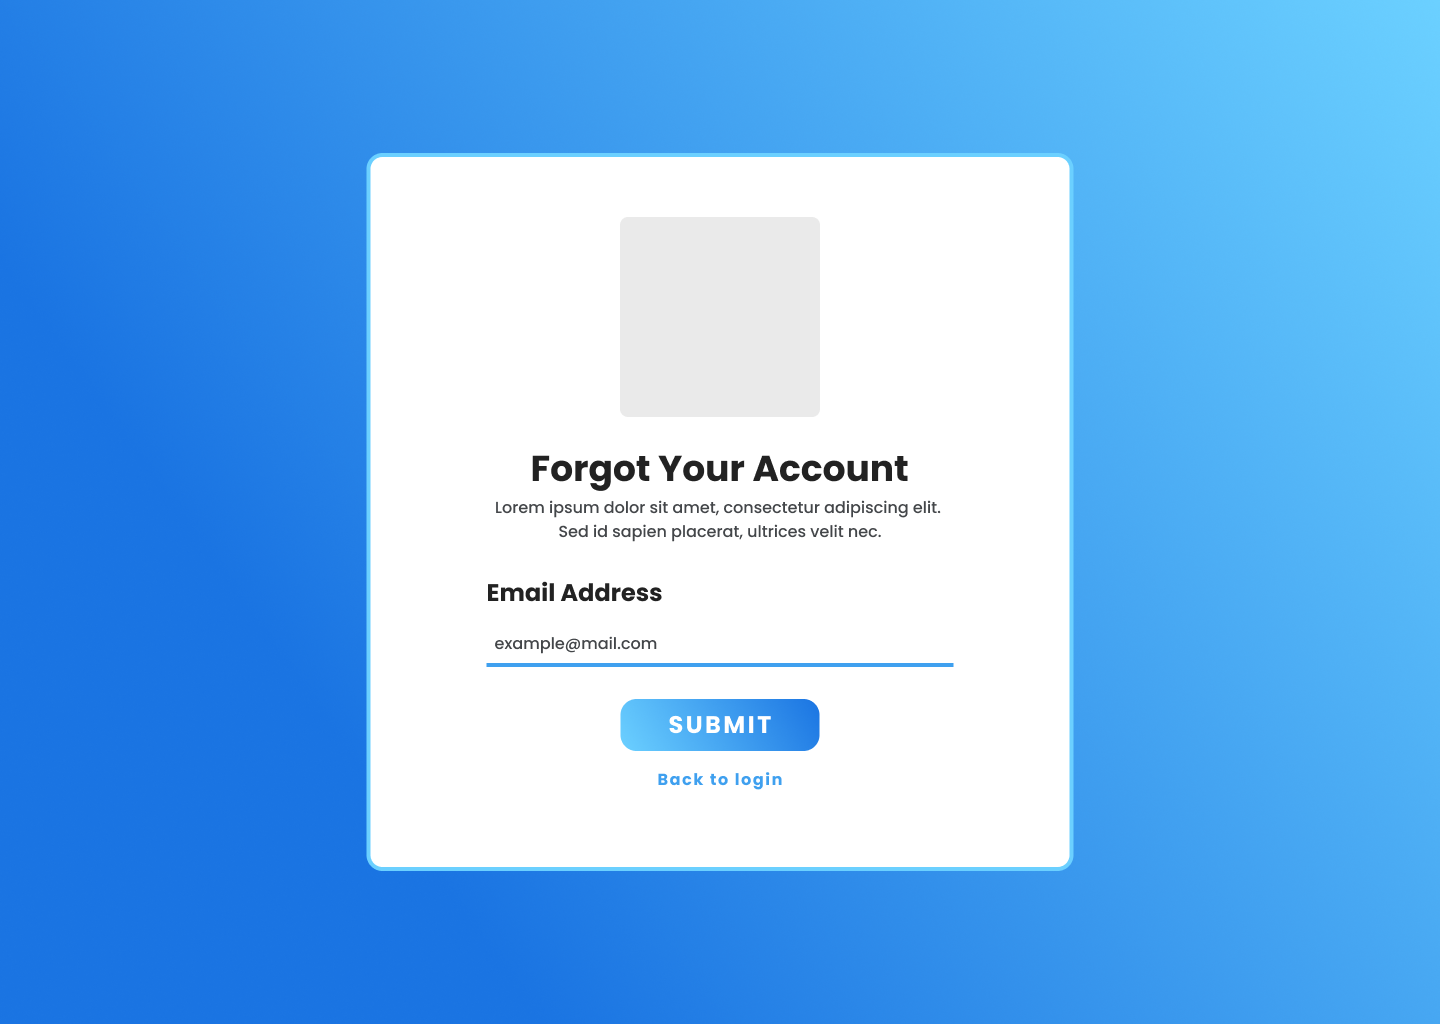
\includegraphics[width= 10cm]{./assets/UI/forgot-password.png}}
\caption{Forgot Password Page}\label{fig:Forgot-Password}
\end{figure}



\begin{figure}[!h]
\centering
\fbox{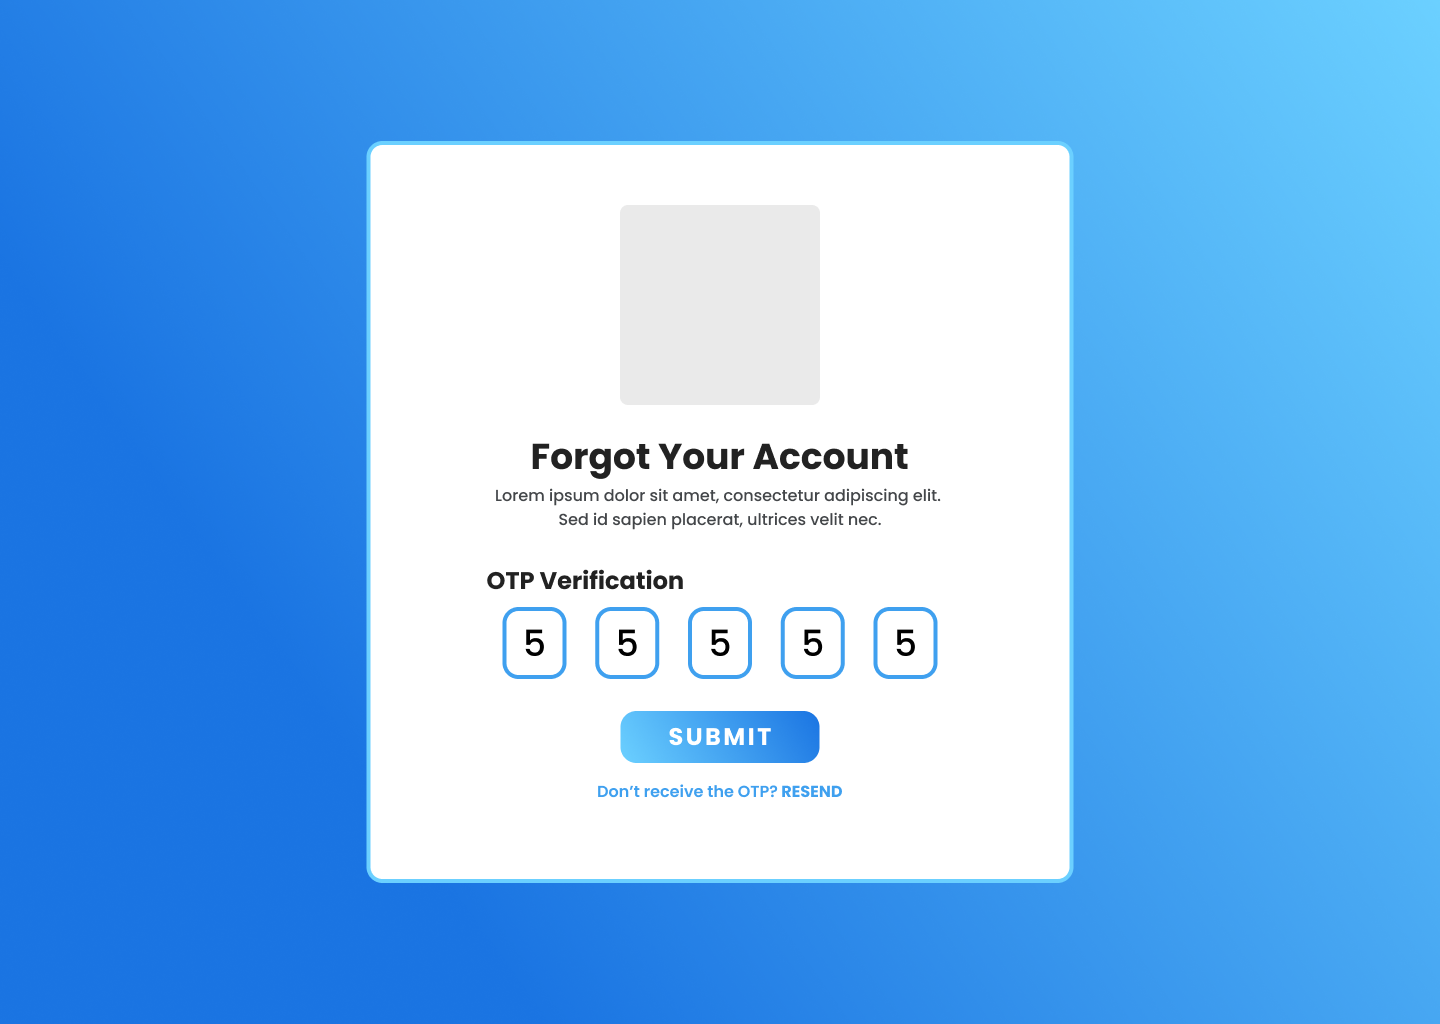
\includegraphics[width= 10cm]{./assets/UI/Forgot-Password-Code.png}}
\caption{Forgot Password Page}\label{fig:Forgot-Password-code}
\end{figure}

\begin{figure}[!h]
\centering
\fbox{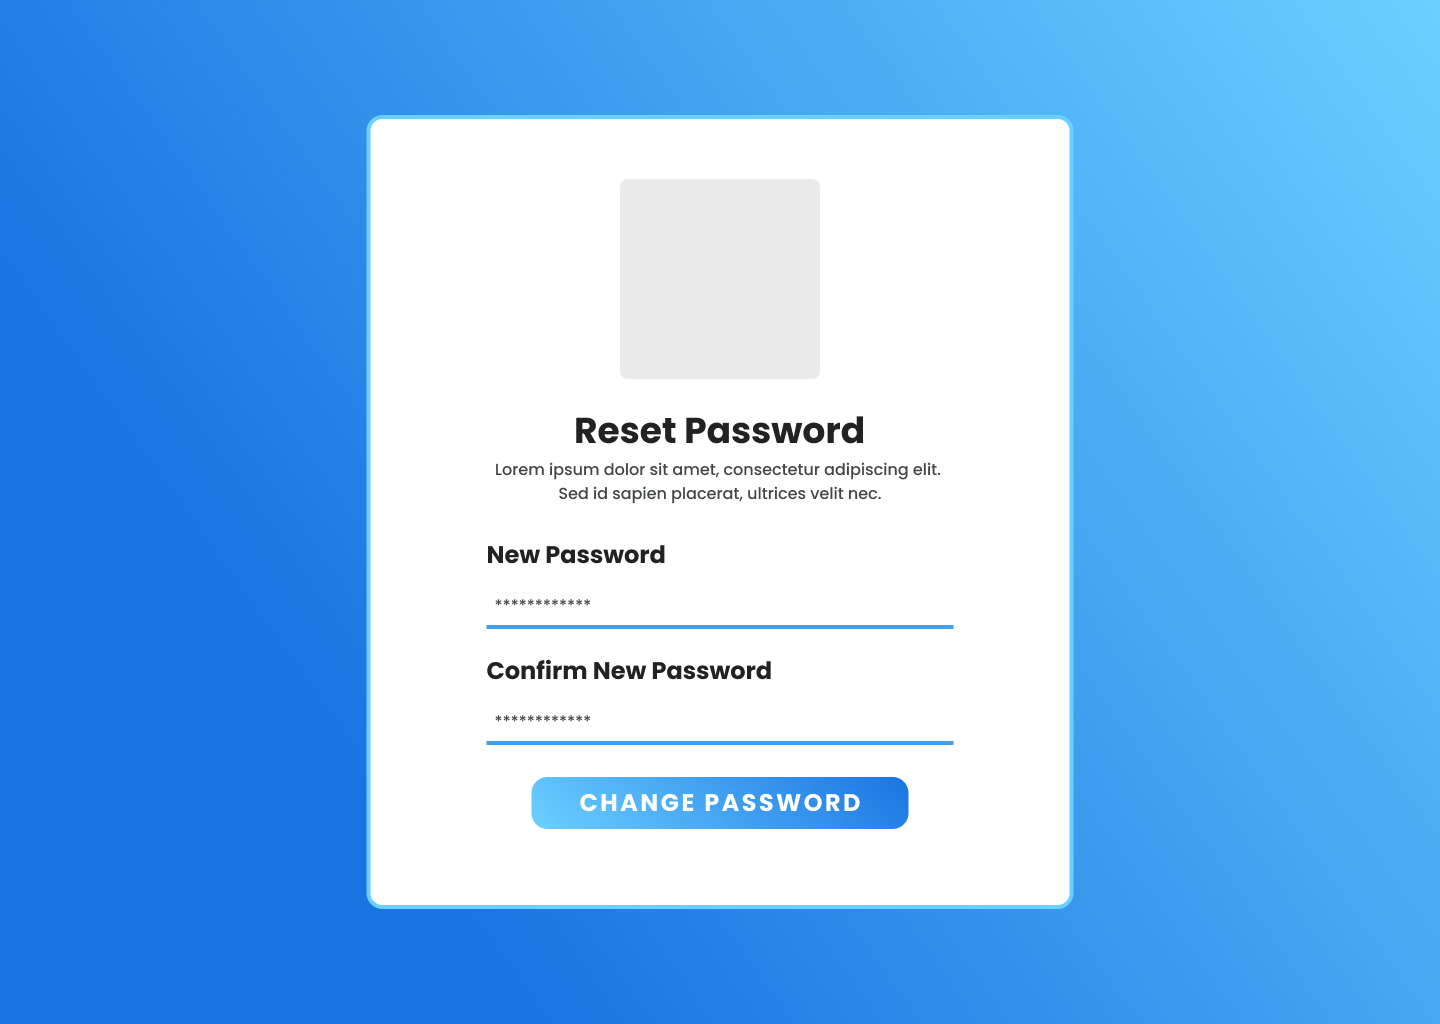
\includegraphics[width= 10cm]{./assets/UI/Reset-password.png}}
\caption{Reset Password Page}\label{fig:Reset Password}
\end{figure}



At the Figure \ref{fig:Forgot-Password-code}, It represents a OTP confirmation page which required a OTP Code that the system have send to the email address. Figure \ref{fig:Reset Password}, It represents a reset password pageIf it success the system will navigate to reset password page for enter a new password.

\newpage
\subsection{Dashboard}

\begin{figure}[!h]
\centering
\fbox{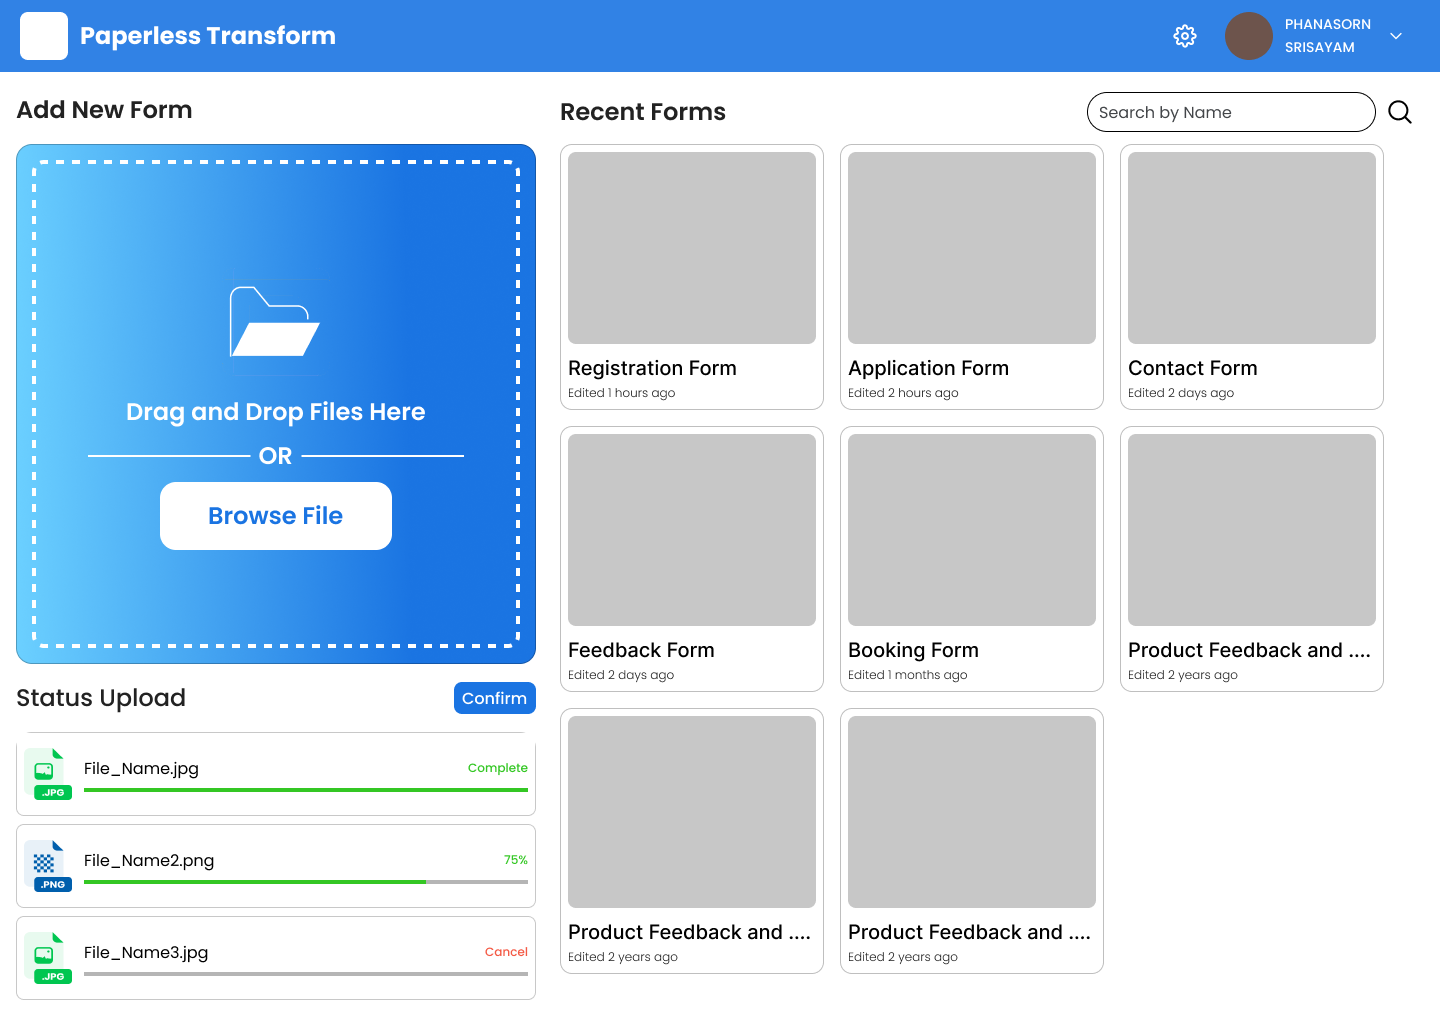
\includegraphics[width= 10cm]{./assets/UI/DashBoard.png}}
\caption{Dashboard Page}\label{fig:Dashboard}
\end{figure}

Figure \ref{fig:Dashboard} represents the dashboard page, it will show all the form that user have and the add form section at the left hand side, also have a upload status while file is uploading.

\newpage
\subsection{Edit Form}

\begin{figure}[!h]
\centering
\fbox{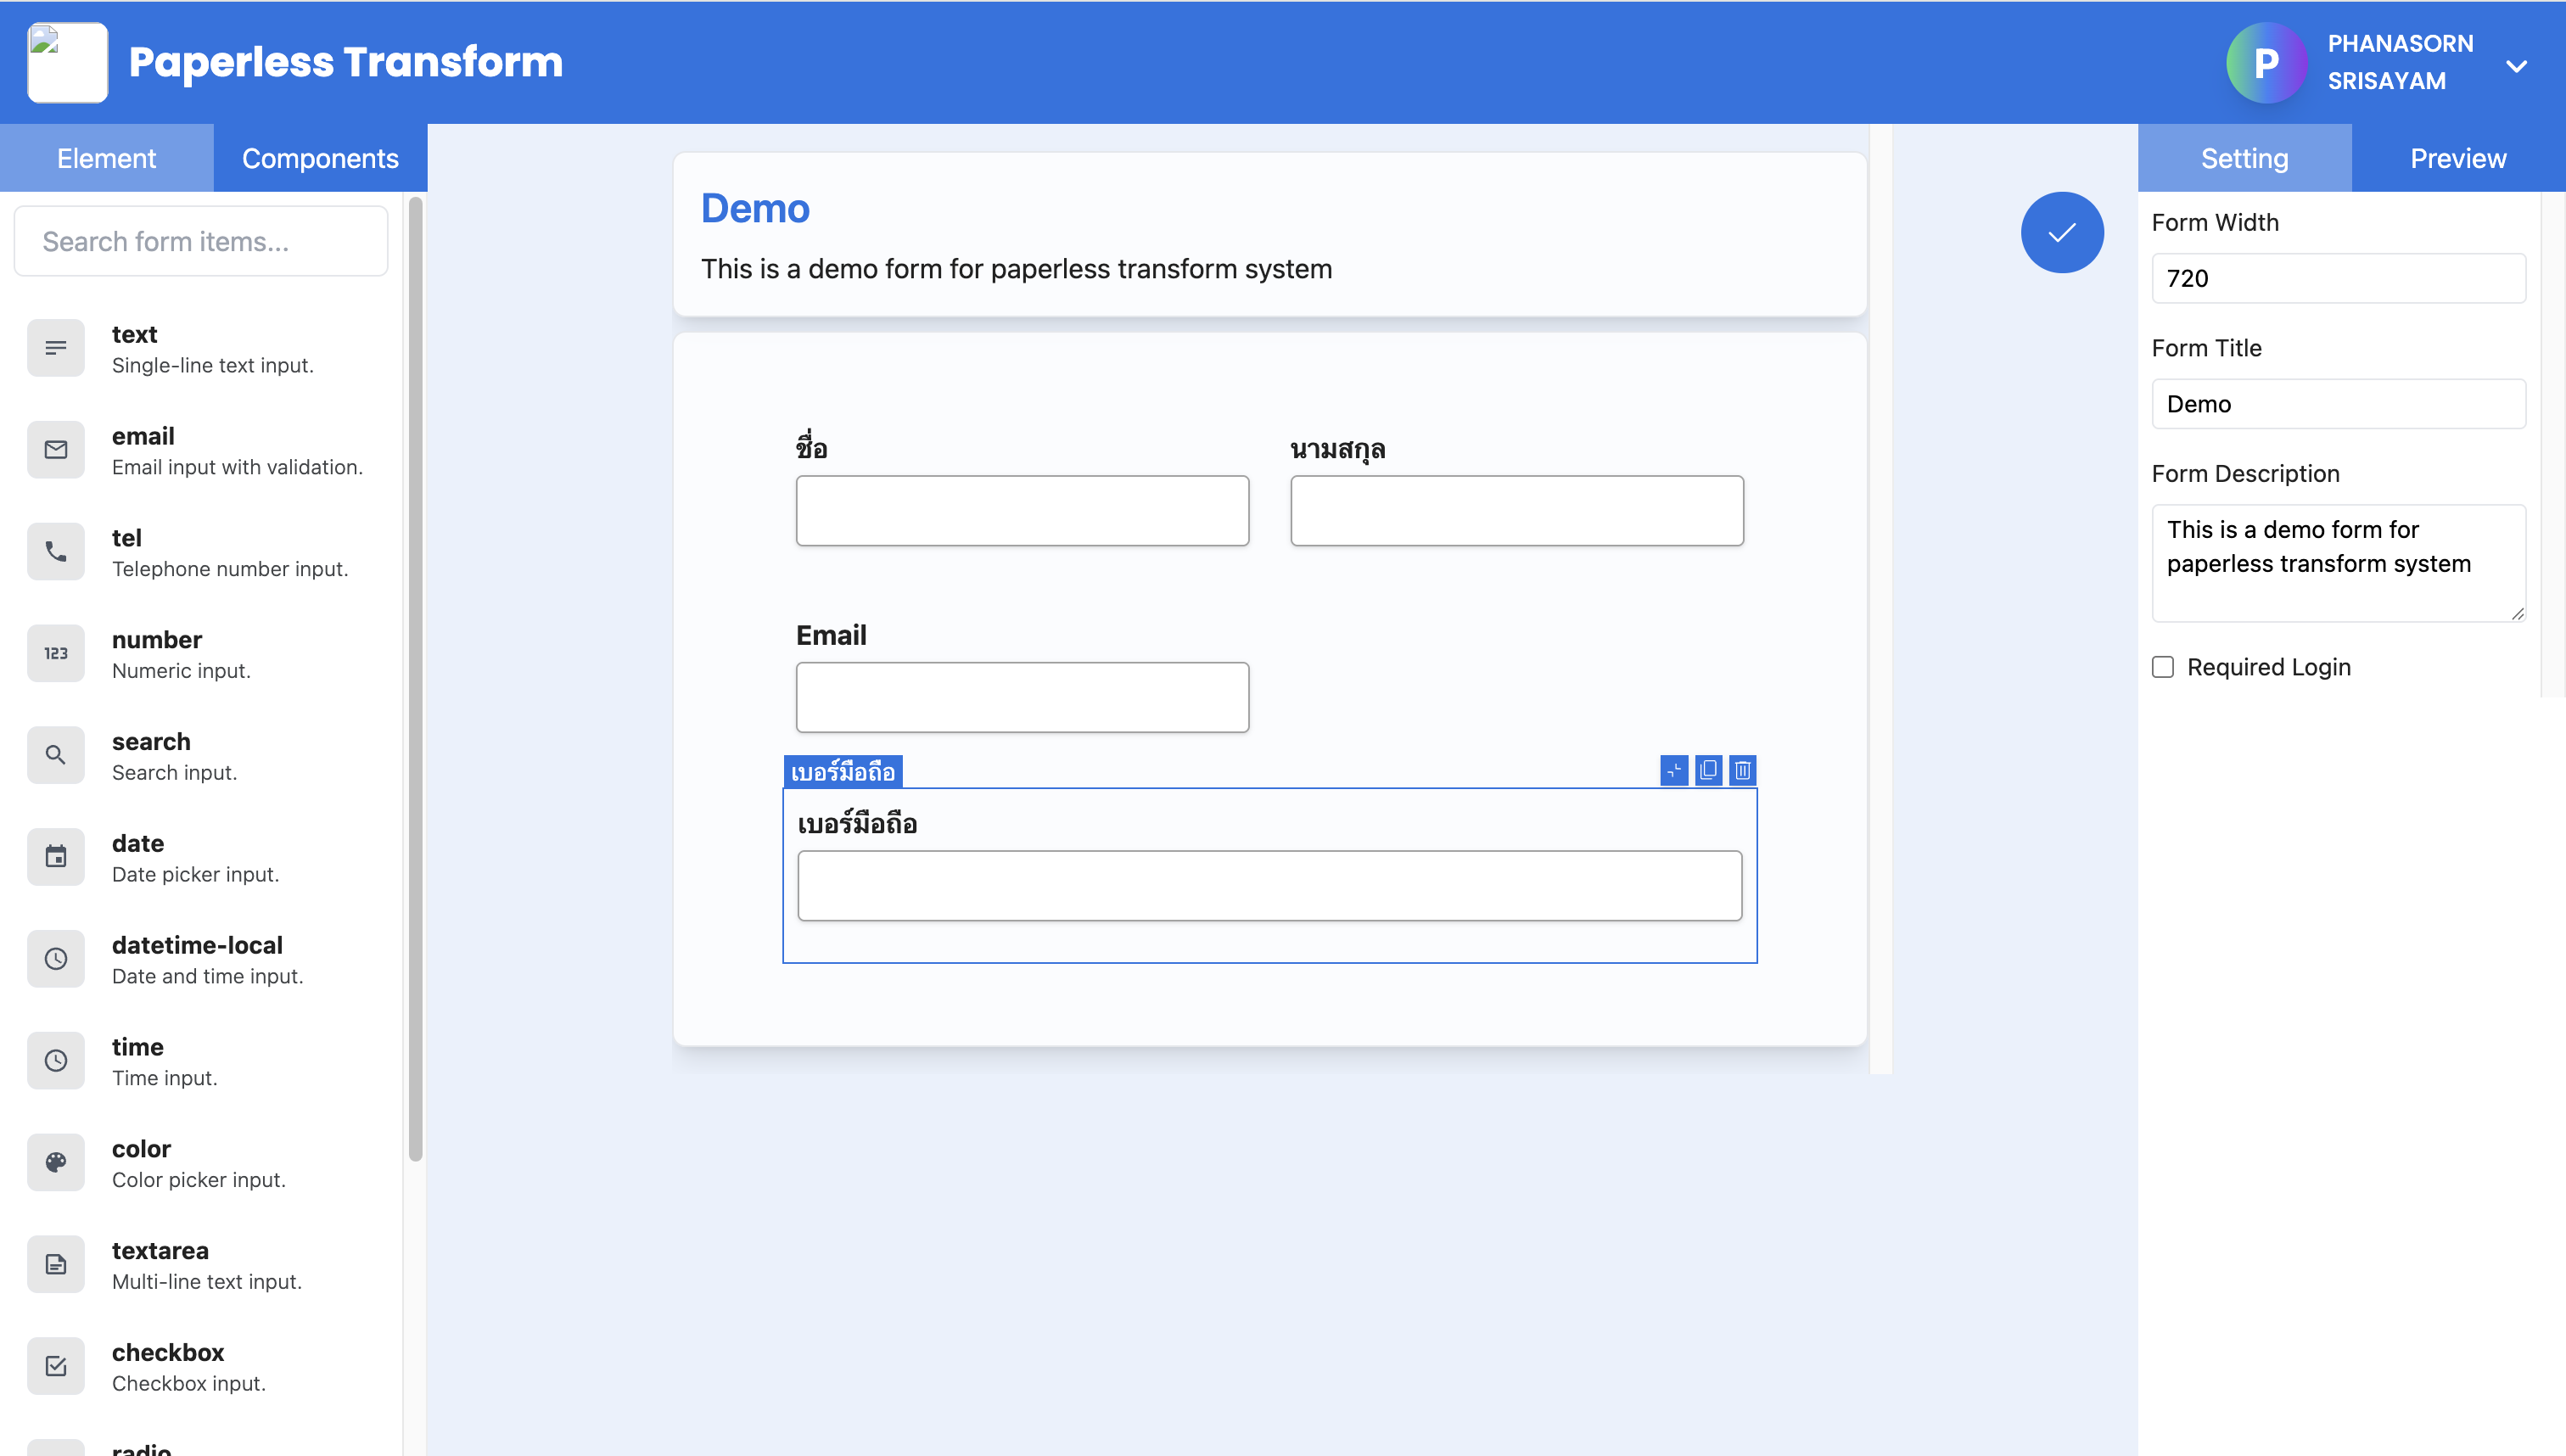
\includegraphics[width= 10cm]{./assets/UI/edit-form.png}}
\caption{Edit Form Page}\label{fig:edit-form}
\end{figure}

Figure \ref{fig:edit-form}  represents the Edit Form. The edit form page uses the SurveyJS library, which allows users to fully customize a form, including changing the color, adding a second page, and creating form conditions.

\subsection{Form Page}

\begin{figure}[!h]
\centering
\fbox{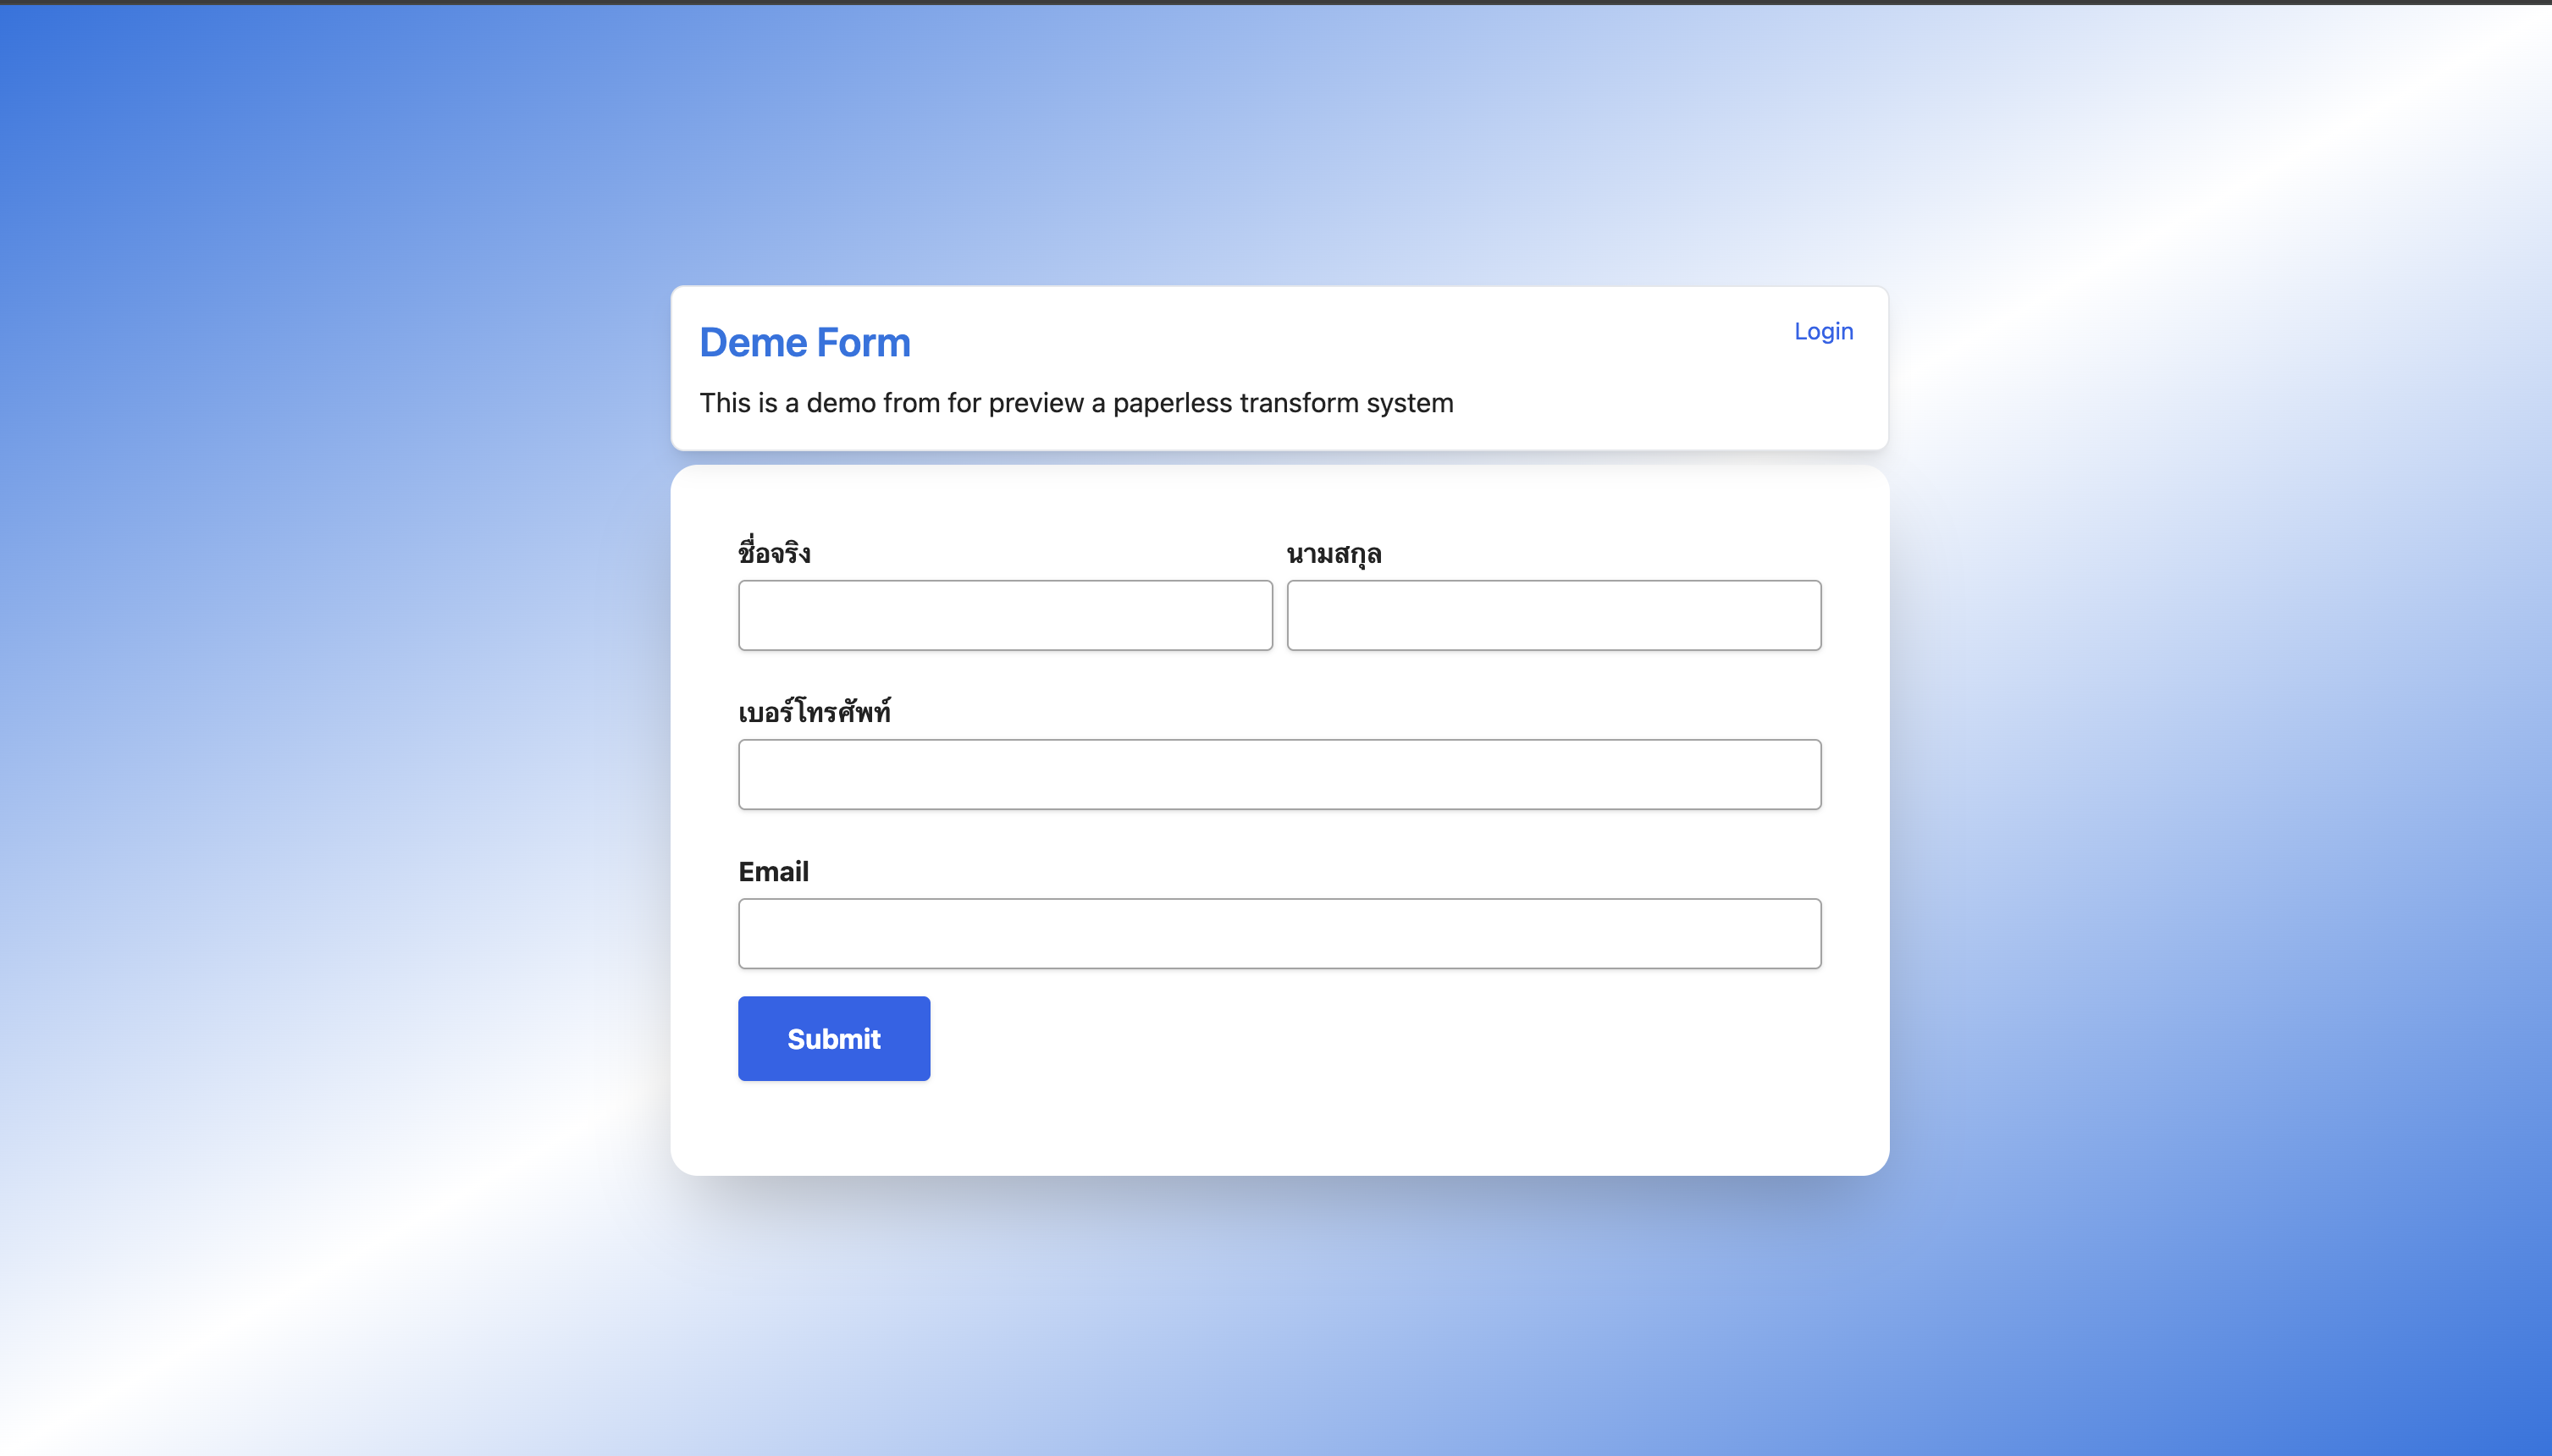
\includegraphics[width= 10cm]{./assets/UI/form-page.png}}
\caption{Form Page}\label{fig:form-page}
\end{figure}

Figure \ref{fig:form-page} showcases the example of web form user interface, which it use a surveyJS to render the UI. This  page will allow user to fill the information and submit a data to the system.


%%%%%%%%%%%%%%%%%%%%%%%%%%%%%%%%%%%%%%%%%%%%%%%%%%%%%%%%%%%%%%
%%%%%%%%%%%%%%%%%%%% Experiments %%%%%%%%%%%%%%%%%%%%%%%%%%%%%
%%%%%%%%%%%%%%%%%%%%%%%%%%%%%%%%%%%%%%%%%%%%%%%%%%%%%%%%%%%%%%%
\chapter{Implementation Result}

This chapter will cover all the working process and implementation progress of our project. also address problems that are challenging. And we will divided each topic by features

\section{Paper-Based Form Analysis System}

The Paper-Based Form Analysis System is mainly focused on extracting a text from the image or file, and analyzing a form layout to identify an input label in the text, also the translation part and data type generator by using generative AI.

\subsection{Text Extraction Feature}
The Text Extraction we have separate into 2 major components which is extraction from image and extraction from PDF. Both of them were implemented already, but there are a problem with the extract text from image because we have use optical character recognition technique and Figure \ref{fig:ocr-result} is a result of the extraction from image, which  contains multiple OCR inaccuracies that affect the readability and accuracy of the extracted text.Character recognition errors are present, where the letter, number and special character are misidentified, such as confusing "O" with "0" or "I" with "1,". And the extraction from PDF is using a PyPlumber to extract text, and the result is working correctly as Figure \ref{fig:pdf-result}.

\begin{figure}[H]
\centering
\fbox{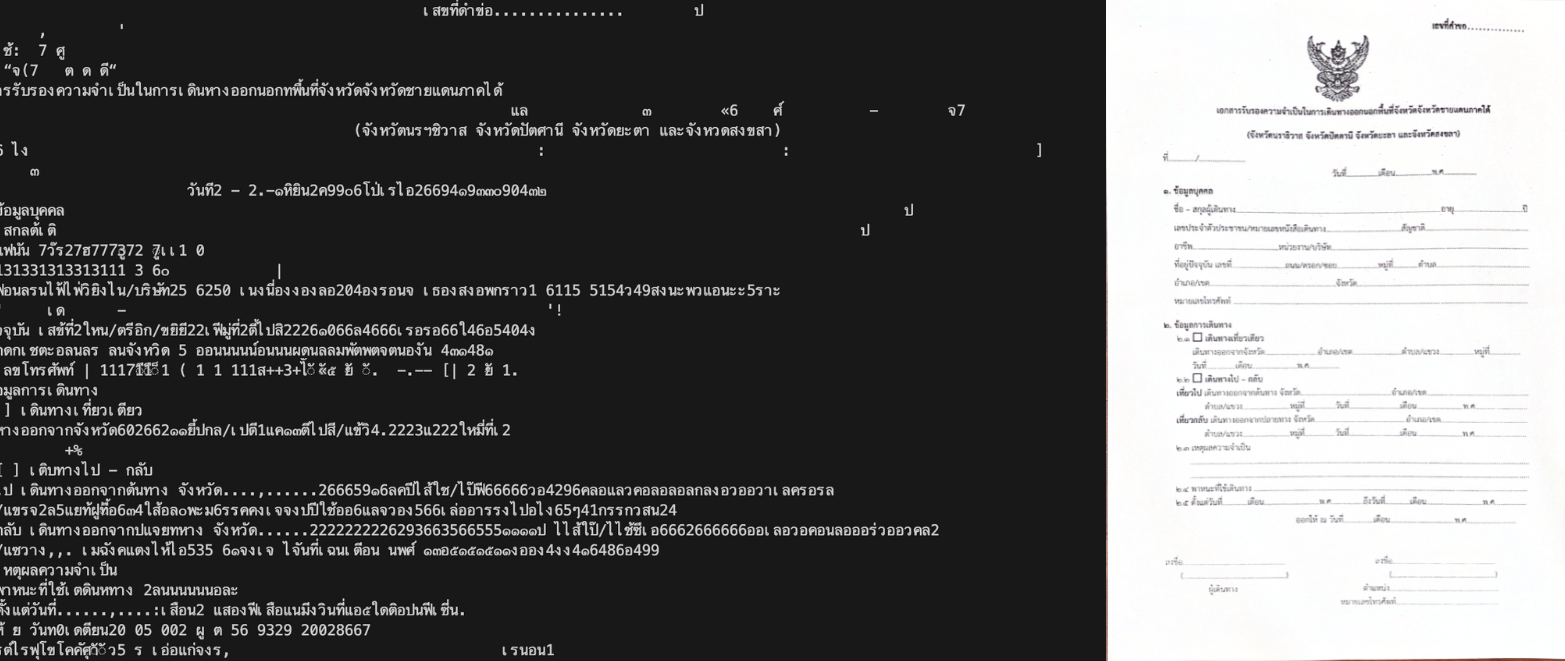
\includegraphics[width= 10cm]{./assets/ocr-result.png}}
\caption{OCR Text Extraction Result}\label{fig:ocr-result}
\end{figure}

\begin{figure}[H]
\centering
\fbox{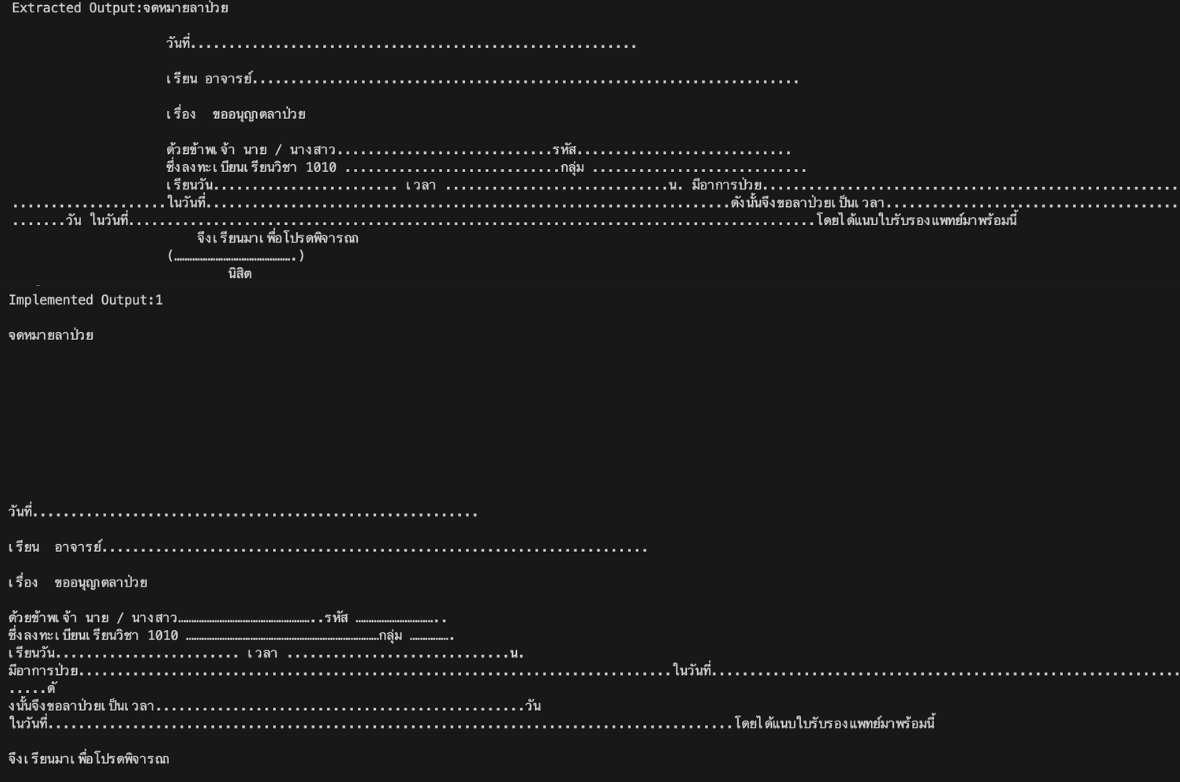
\includegraphics[width= 10cm]{./assets/pdf-extract.png}}
\caption{PDF Text Extraction Result}\label{fig:pdf-result}
\end{figure}

\subsection{Form Parse}
The Form Parse is implemented to identify an input label of the form and separate a form title. we have tested a several form and the result of form parse was 
great but there are some minor defects, if the extracted text does not match with the pattern algorithm that we design, so some labels may be missing.

\begin{figure}[H]
\centering
\fbox{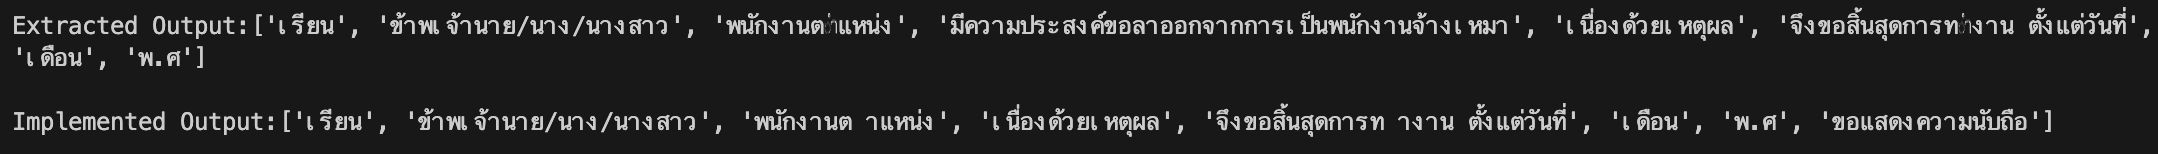
\includegraphics[width= 10cm]{./assets/form-parse.png}}
\caption{Form Parse Result}\label{fig:Form-Parse}
\end{figure}

\subsection{Translation Thai to English}
The Translation is use to translate a Thai language input label to english. we have use a NLLB-200 fined tuned model. Figure \ref{fig:trans-result} below show that the translation is working correctly but may not it may get a text that we expect, such as \textthai{วันเกิด} expected value to be Date of Birth, but the predicted result show "Birthdate". which it have ability to translate into a correct meaning.

\begin{figure}[H]
\centering
\fbox{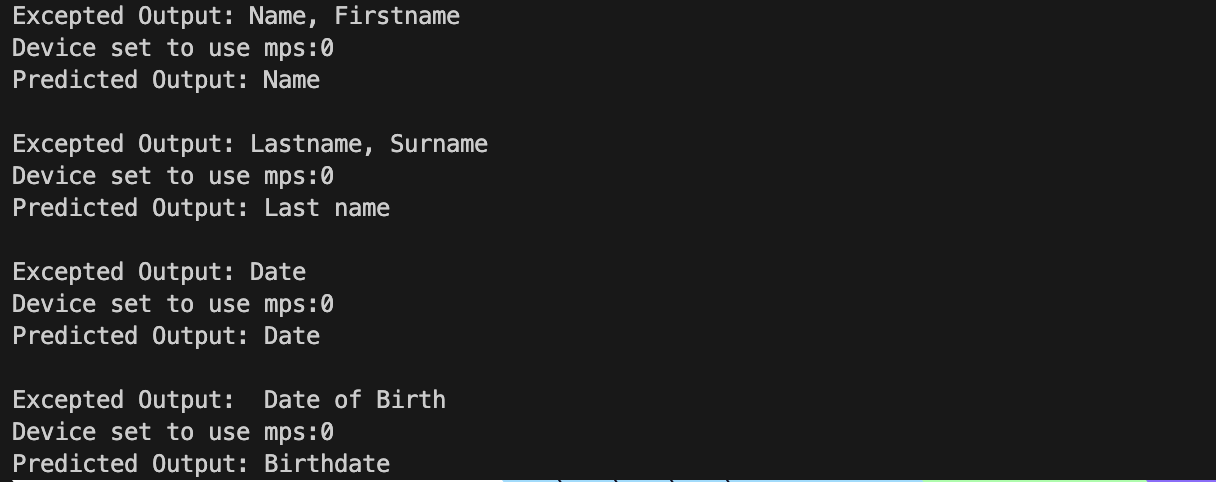
\includegraphics[width= 10cm]{./assets/translation-result.png}}
\caption{Translation Result}\label{fig:trans-result}
\end{figure}

\subsection{Data Type Analyzer}
Figure \ref{fig:datatype-result} has shown the 3 simple test case result that input the array of text and the system will generate a json as output. And it show a correct result for 1 and 2, but the 3 has failed because we have input a Thai text and some field are not correct as expect result.

\begin{figure}[H]
\centering
\fbox{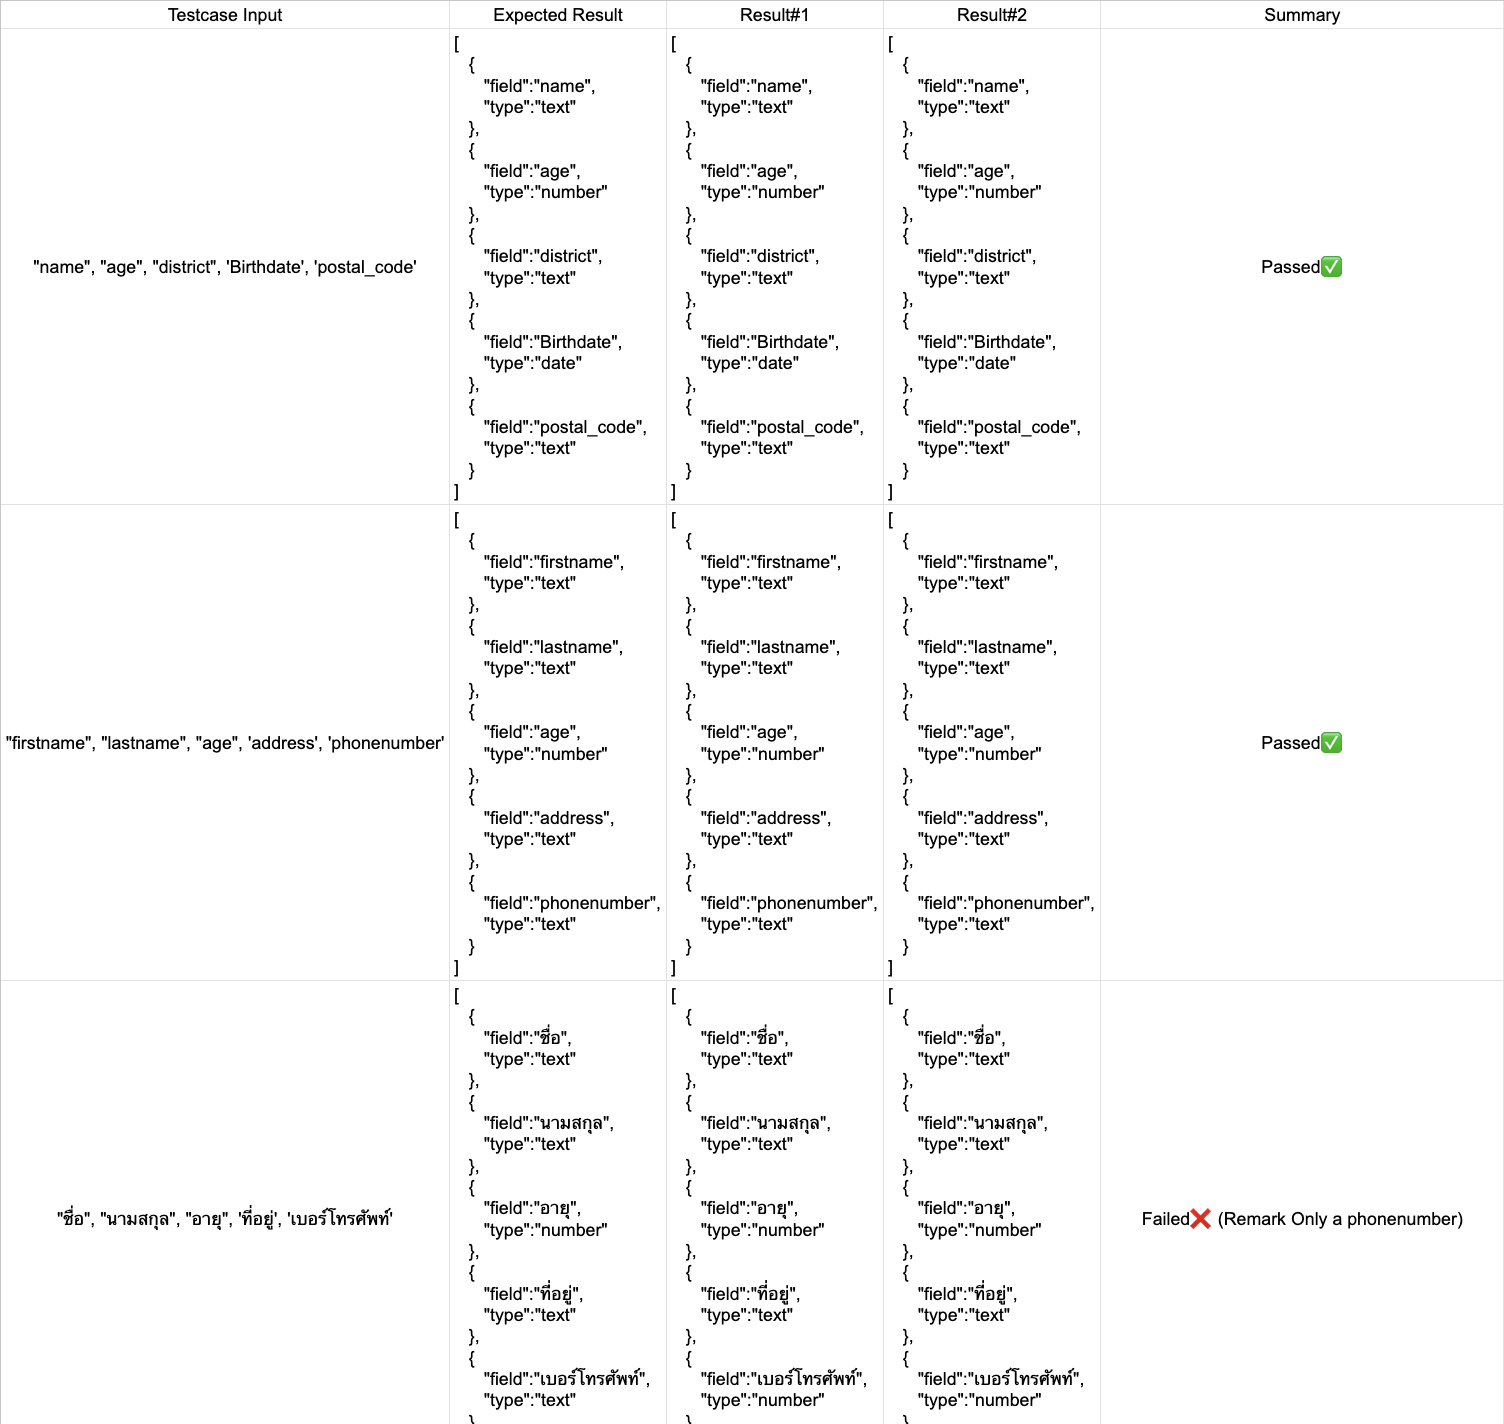
\includegraphics[width= 10cm]{./assets/datatype-result.png}}
\caption{Data Type Analyzer Result}\label{fig:datatype-result}
\end{figure}


\section{Web Application Implementation}

The web application development is progressing well, with significant milestones achieved in the front-end implementation. The following features have been successfully developed and tested with a responsive user interface.

\textbf{Authentication System:} Includes Login, Sign-Up, and Forgot Password pages.

\begin{figure}[H]
\centering
\fbox{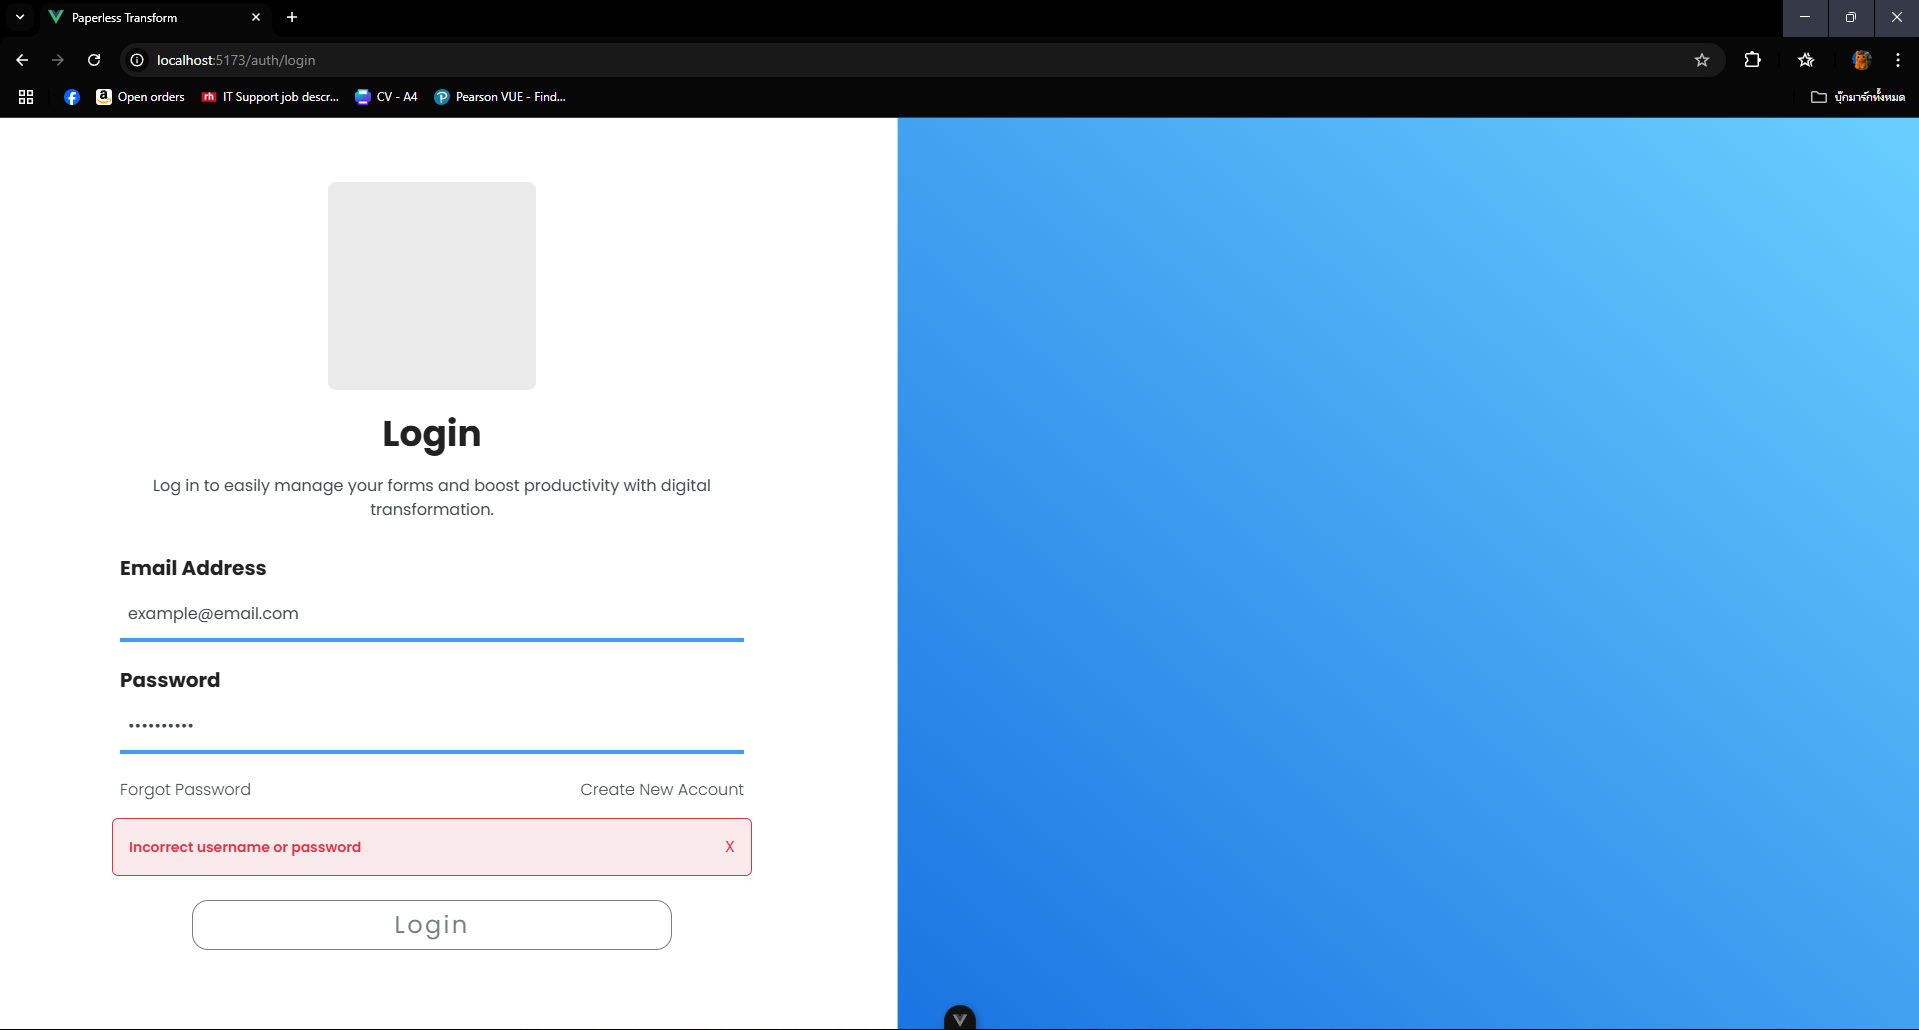
\includegraphics[width= 10cm]{./assets/auth-login.png}}
\caption{Implemented Login Page}\label{fig:auth-login}
\end{figure}

\begin{figure}[H]
\centering
\fbox{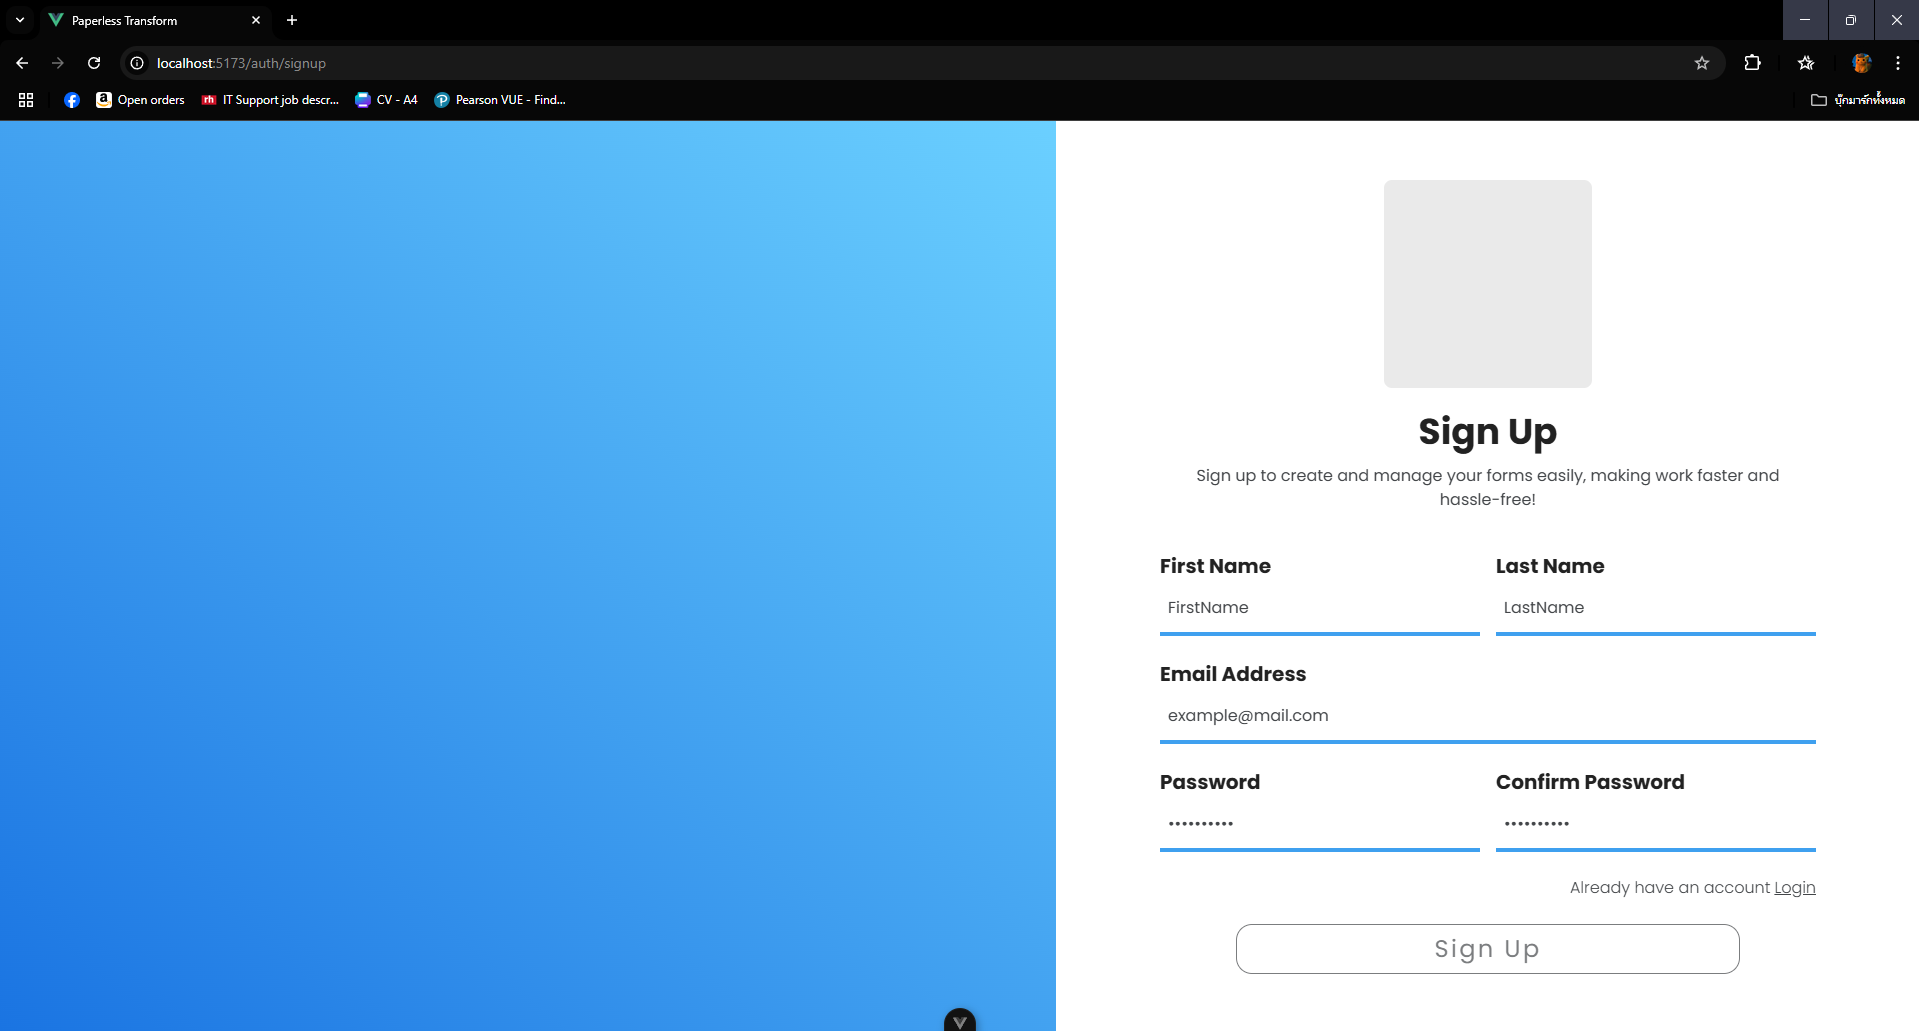
\includegraphics[width= 10cm]{./assets/auth-signup.png}}
\caption{Implemented Signup Page}\label{fig:auth-signup}
\end{figure}

\begin{figure}[H]
\centering
\fbox{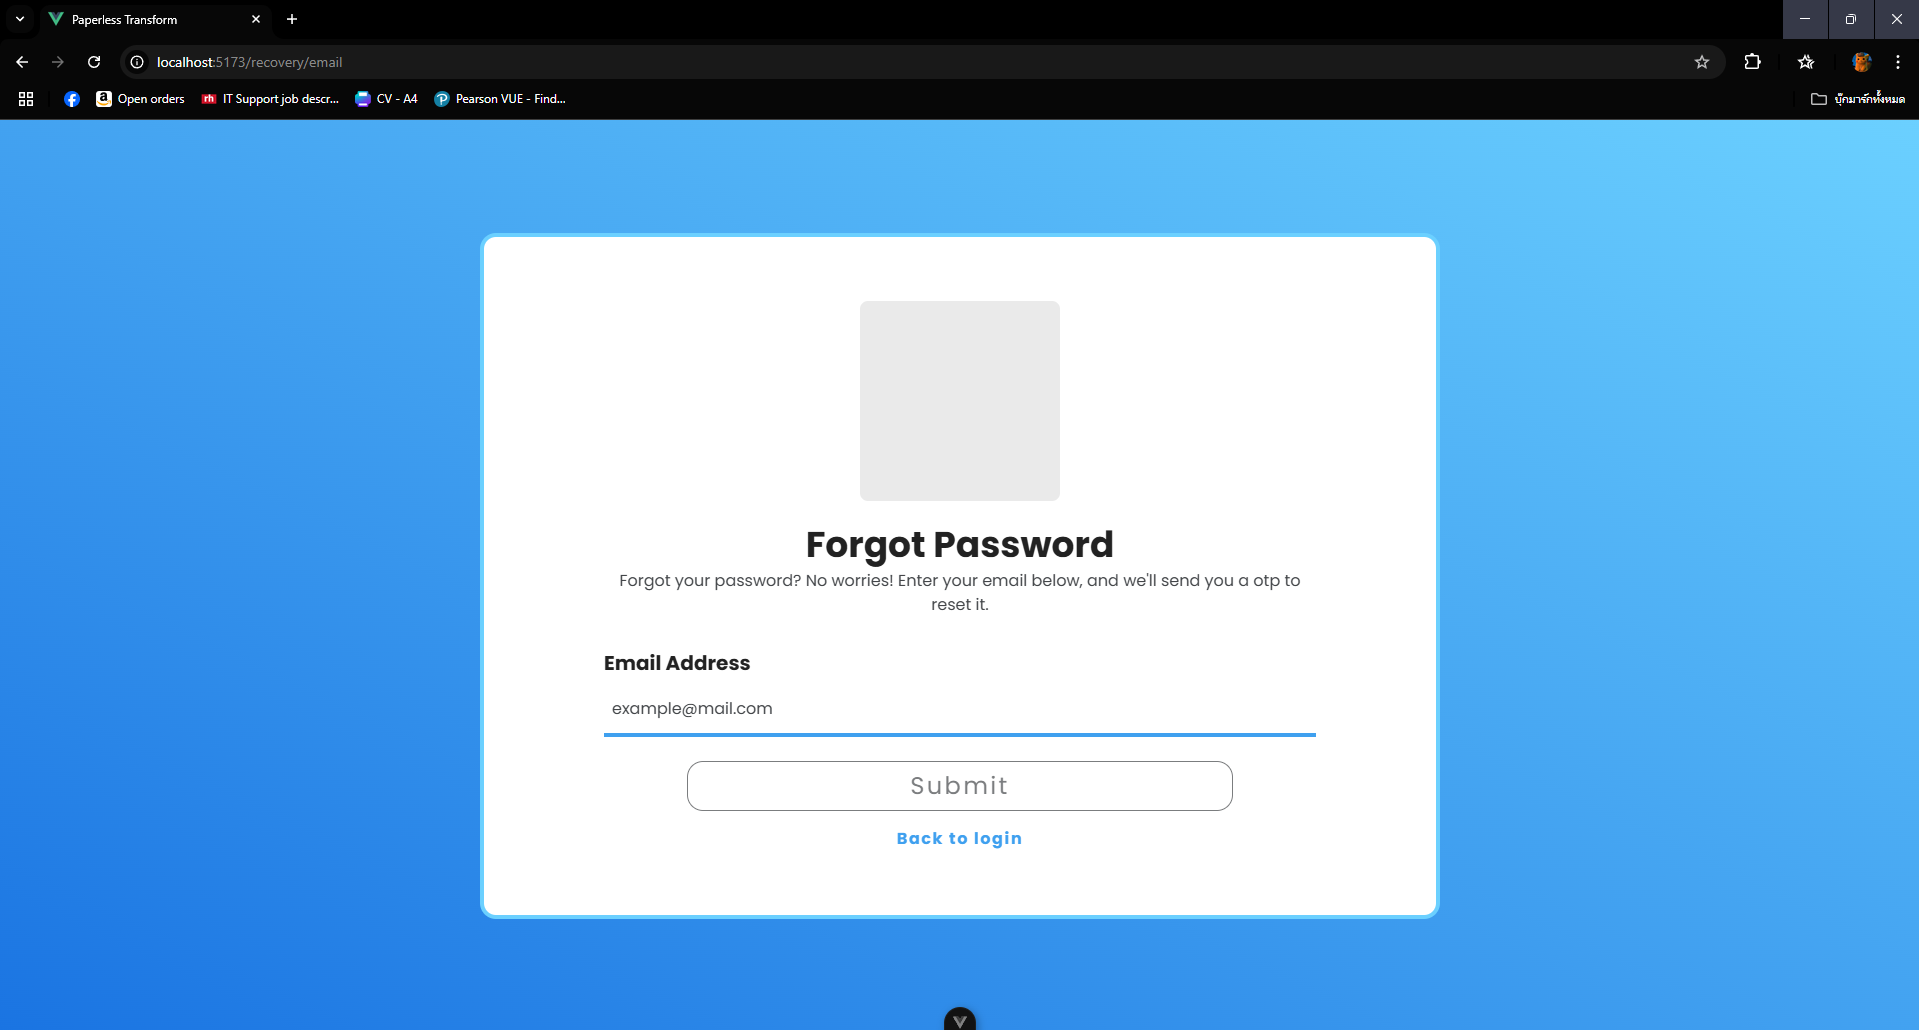
\includegraphics[width= 10cm]{./assets/auth-forgotpasswd.png}}
\caption{Implemented Forgot Passowrd}\label{fig:auth-forgotpasswd}
\end{figure}

\textbf{Dashboard Page:} Dashboard Page: Fully implemented with necessary functionalities,  such as upload files, status files upload, and recent form display with search by keyword.

\begin{figure}[H]
\centering
\fbox{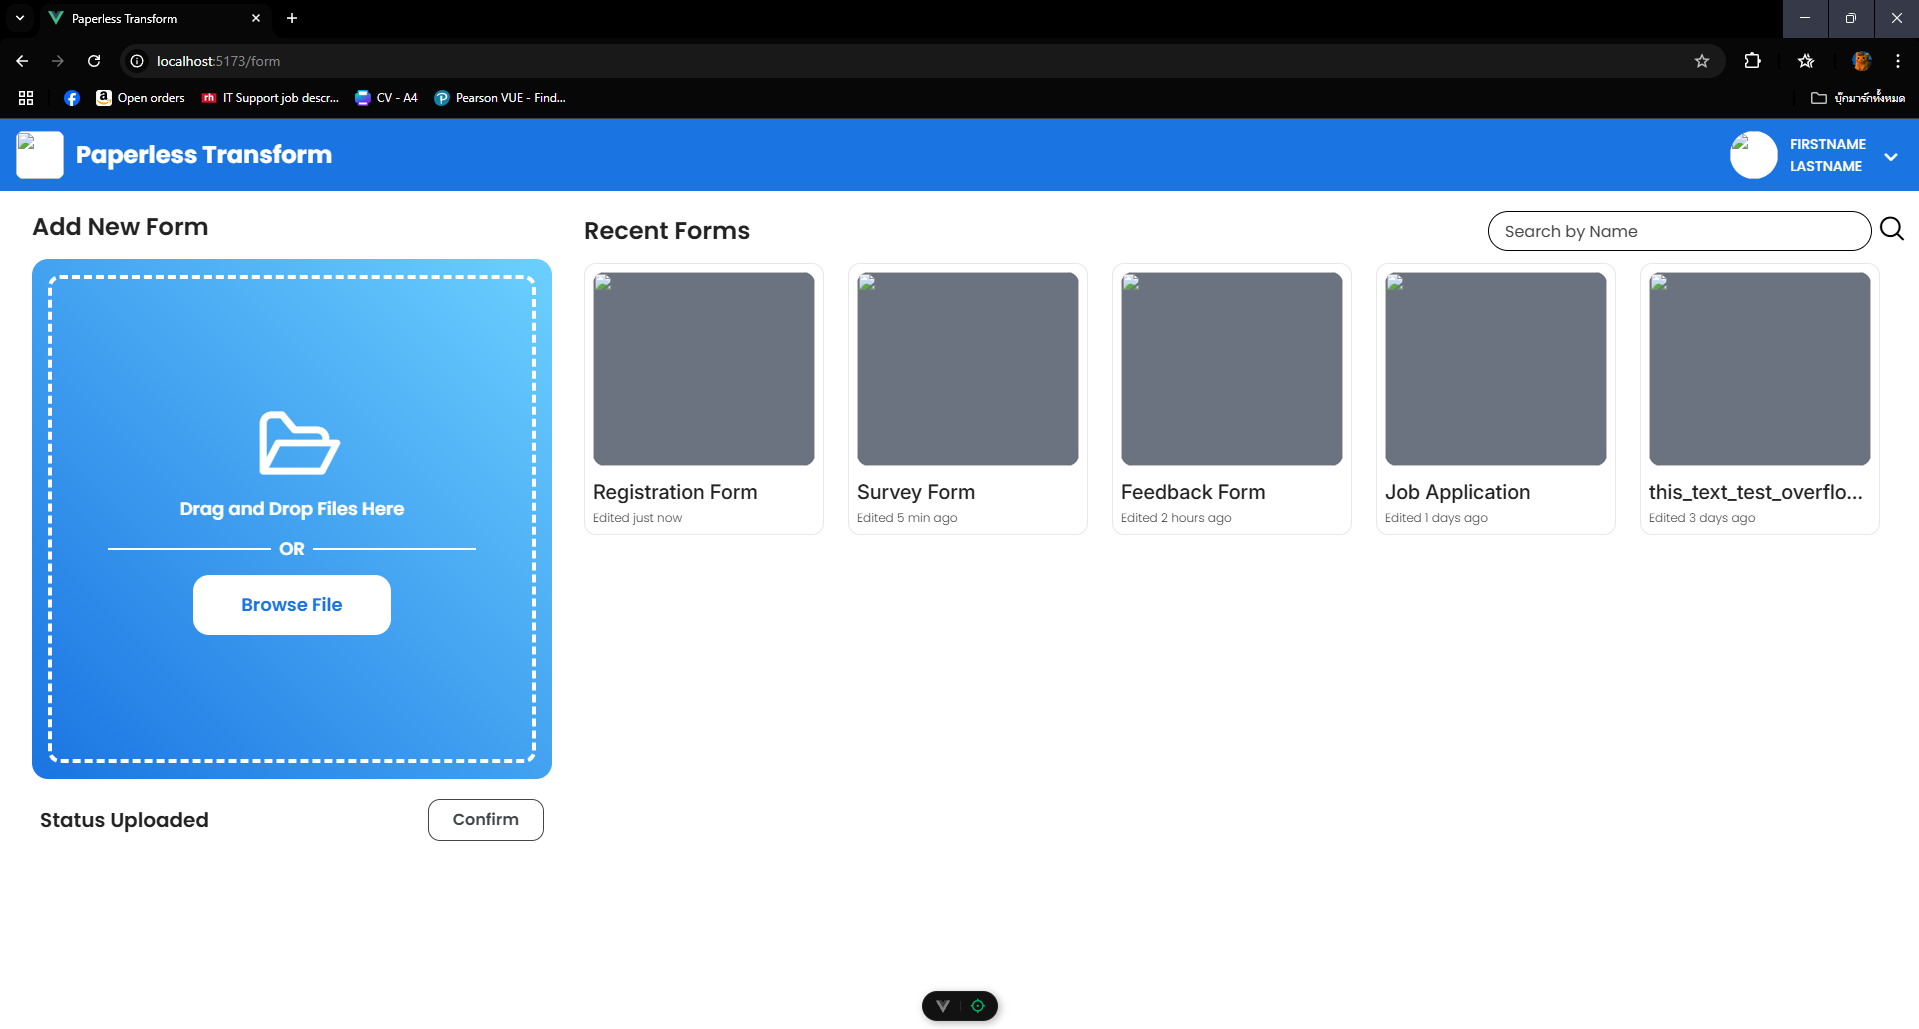
\includegraphics[width= 10cm]{./assets/dashboard.png}}
\caption{Implemented Dashboard Page}\label{fig:dashboard-result}
\end{figure}

%%%%%%%%%%%%%%%%%%%%%%%%%%%%%%%%%%%%%%%%%%%%%%%%%%%%%%%%%%%%%%%
%%%%%%%%%%%%%%%%%%%% Conclusions %%%%%%%%%%%%%%%%%%%%%%%%%%%%%
%%%%%%%%%%%%%%%%%%%%%%%%%%%%%%%%%%%%%%%%%%%%%%%%%%%%%%%%%%%%%%%
%\chapter{Conclusions}

 %\begin{figure}[!h]
%\caption{This is how you mention when figure come from internet  \href{https://www.google.com} {https://www.google.com}}\label{fig:x1}
%\end{figure}

%This chapter is optional for proposal and progress reports but 
%is required for the final report.

%THIS IS AN EXAMPLE. ALL SECTIONS BELOW ARE OPTIONAL. PLEASE CONSULT YOU ADVISOR AND DESIGN YOUR OWN SECTION

%\emph{\textthai{หัวข้อต่าง ๆ ในแต่ละบทเป็นเพียงตัวอย่างเท่านั้น หัวข้อที่จะใส่ในแต่ละบทขึ้นอยู่กับโปรเจคของนักศึกษาและอาจารย์ที่ปรึกษา}}

%\section{Problems and Solutions}
%State your problems and how you fixed them.

%\section{Future Works}
%What could be done in the future to make your projects better.

%%%%%%%%%%%%%%%%%%%%%%%%%%%%%%%%%%%%%%%%%%%%%%%%%%%%%%%%%%%%%%%
%%%%%%%%%%%%%%%%%%%% Bibliography %%%%%%%%%%%%%%%%%%%%%%%%%%%%%
%%%%%%%%%%%%%%%%%%%%%%%%%%%%%%%%%%%%%%%%%%%%%%%%%%%%%%%%%%%%%%%

%%%% Comment this in your report to show only references you have
%%%% cited. Otherwise, all the references below will be shown.
%\nocite{*}
%% Use the kmutt.bst for bibtex bibliography style 
%% You must have cpe.bib and string.bib in your current directory.
%% You may go to file .bbl to manually edit the bib items.

% Sept, 2021 by Thanin
% improve url breaks to prevent unnecessary big white spaces in some cases
\makeatletter
\g@addto@macro{\UrlBreaks}{\UrlOrds}
\makeatother
% 

\bibliographystyle{kmutt}
\bibliography{string,cpe}

\end{document}
